\documentclass{../source/zjureport}

\major{信息工程}
 \name{箫宇 }
\title{实验设计报告}
\stuid{ }
\college{信息与电子工程学院}
\date{\today}
\lab{东4-221}
\course{电磁场与电磁波}
\instructor{王子立}
\grades{}
\expname{实验设计报告}
\exptype{测试实验}
\partner{}

\begin{document}
    \makecover
    \makeheader
    
    \part{CST仿真}
    \section{实验目的}
        \begin{enumerate}
            \item 了解并掌握波导喇叭天线的常用参数指标和分析方法。
            \item 熟悉CST软件的基本操作流程,并能够运用其对特定的微波器件或电路进行建模、仿真分析。
        \end{enumerate}
    \section{实验要求}
        \subsection{喇叭尺寸}
        \begin{enumerate}
            \item 角锥喇叭天线尺寸:$D_H = 80mm , D_E = 38mm , L = 80mm$
            \item 波导尺寸:$a = 22.86mm , b = 10.16mm , Lambda = 29.1mm$
            \item 铜壁厚:$t = 1mm$
        \end{enumerate}
        \subsection{实验任务}
        用 CST软件建模并仿真,观察方向图和喇叭中电场等情况。
        \begin{enumerate}
            \item 分析喇叭天线的方向图,和理论计算的异同。
            \item 分析喇叭天线S11 和驻波比特性曲线。
            \item 分析说明喇叭天线和波导口的电场情况。
        \end{enumerate}

    \section{实验步骤}
        \subsection{制作喇叭模型}
        \newpage
            \subsubsection{新建工程}
            \begin{figure}[thp]
                \centering
                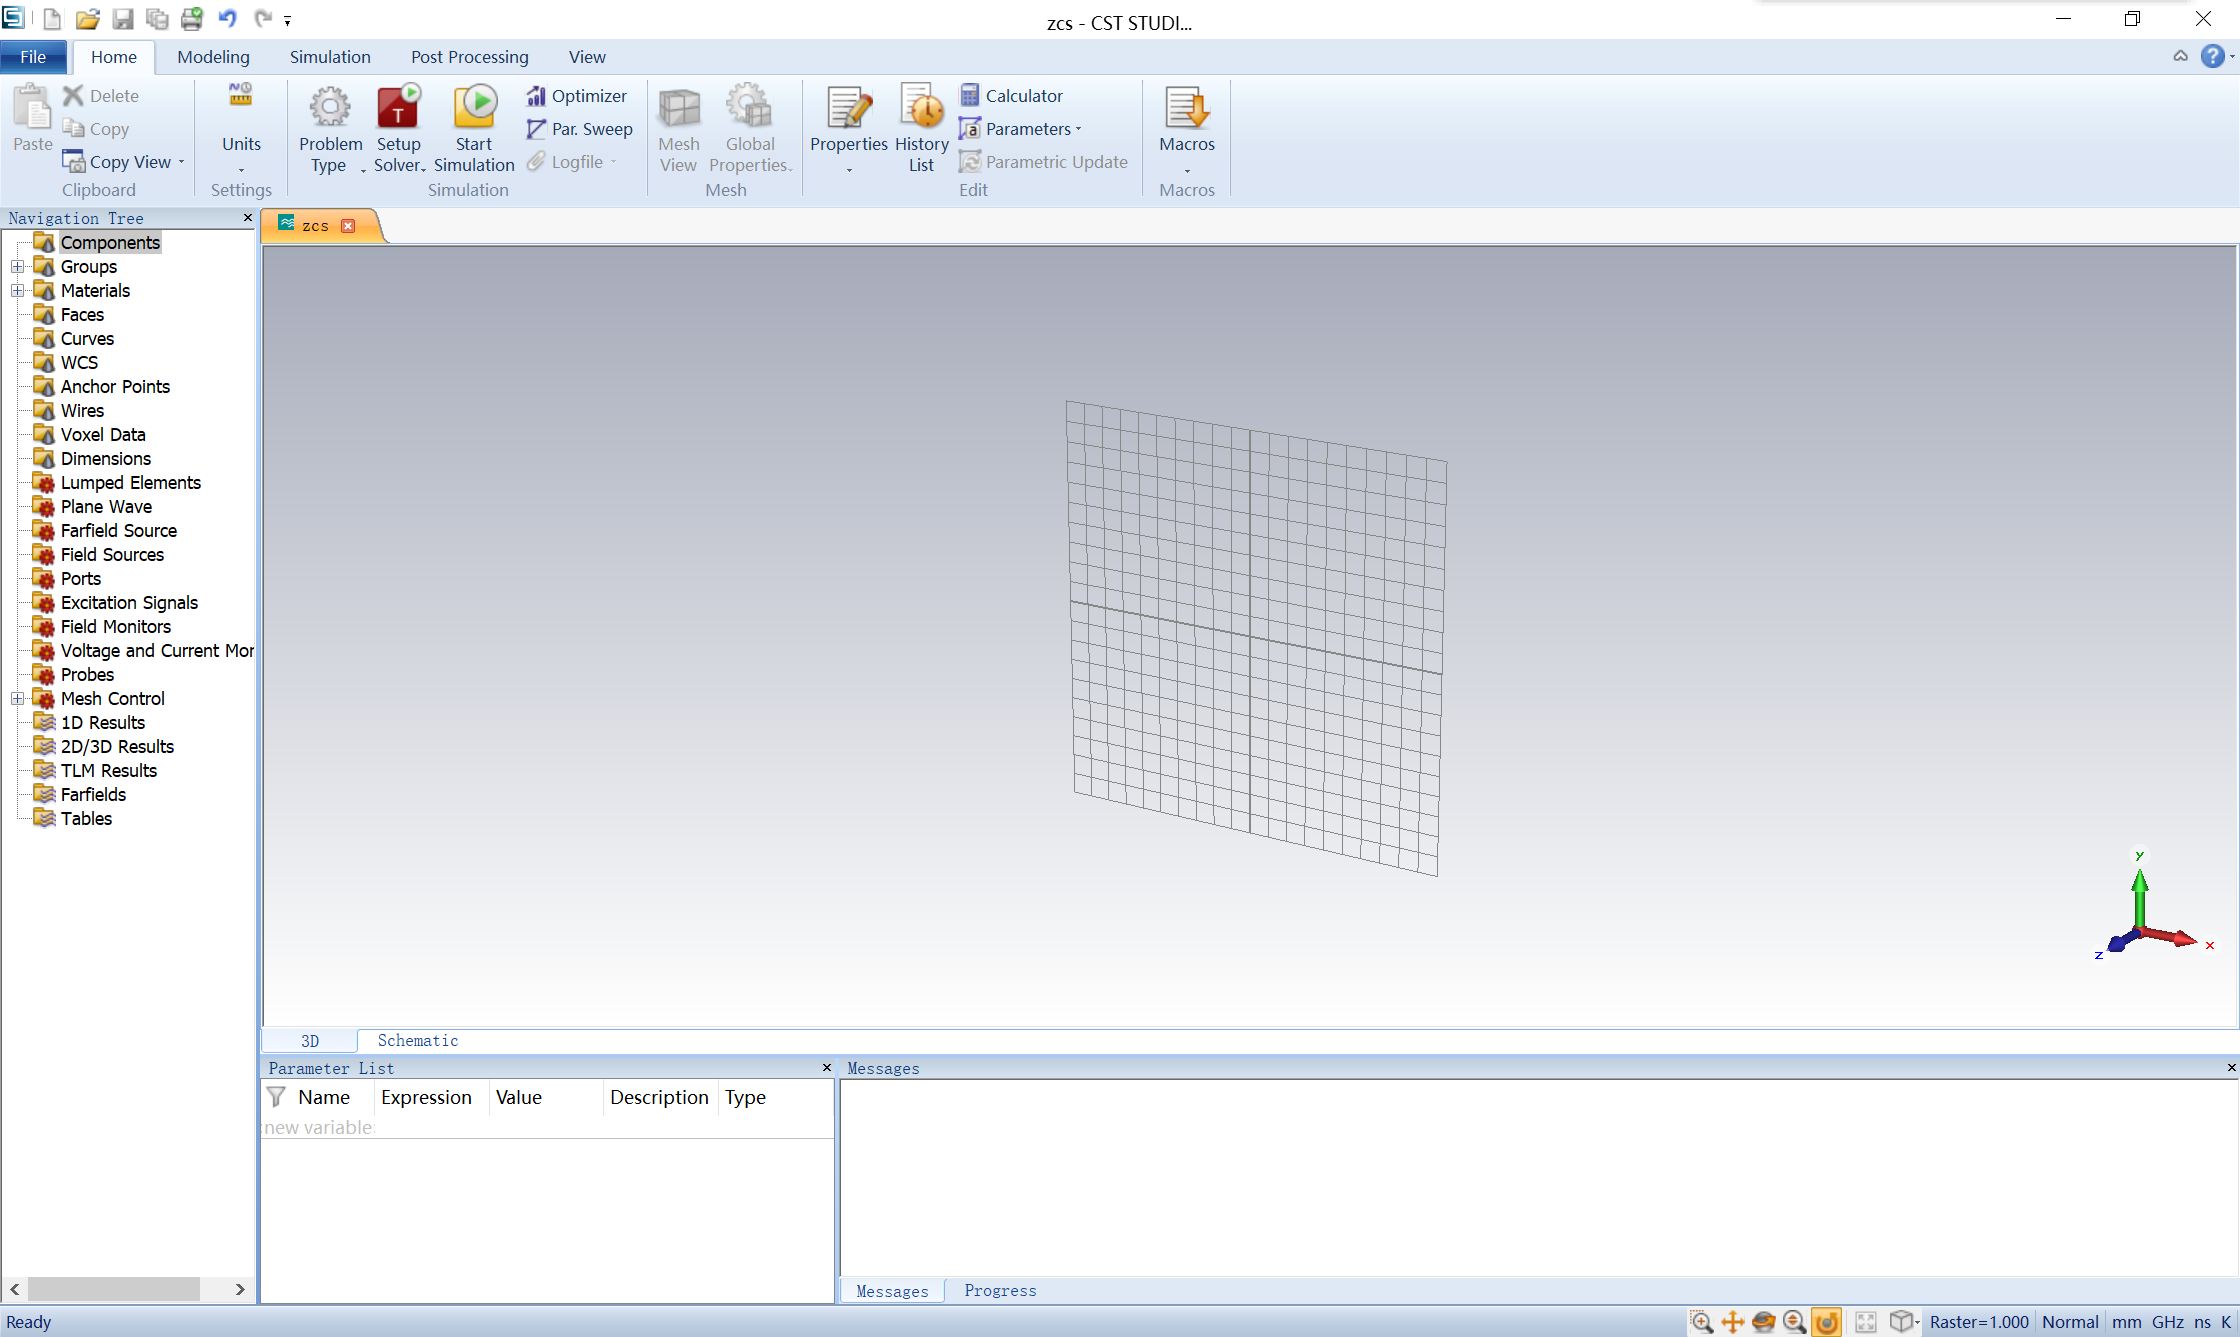
\includegraphics[width = 0.8\textwidth]{figure/1.png}
            \end{figure}
            \subsubsection{创建矩形}
            \begin{figure}[thp]
                \centering
                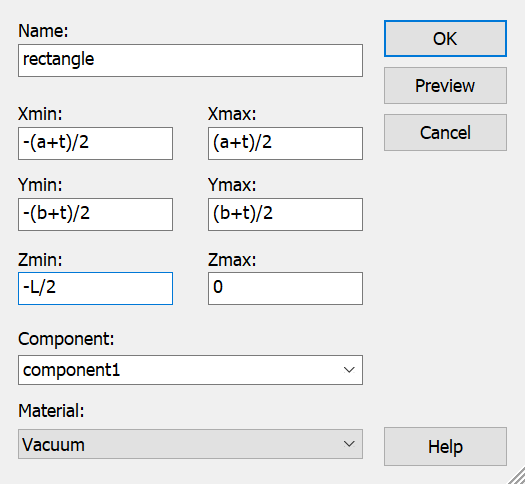
\includegraphics[width = 0.5\textwidth]{figure/矩形参数.png}
            \end{figure}
            \newpage
            \begin{figure}[thp]
                \centering
                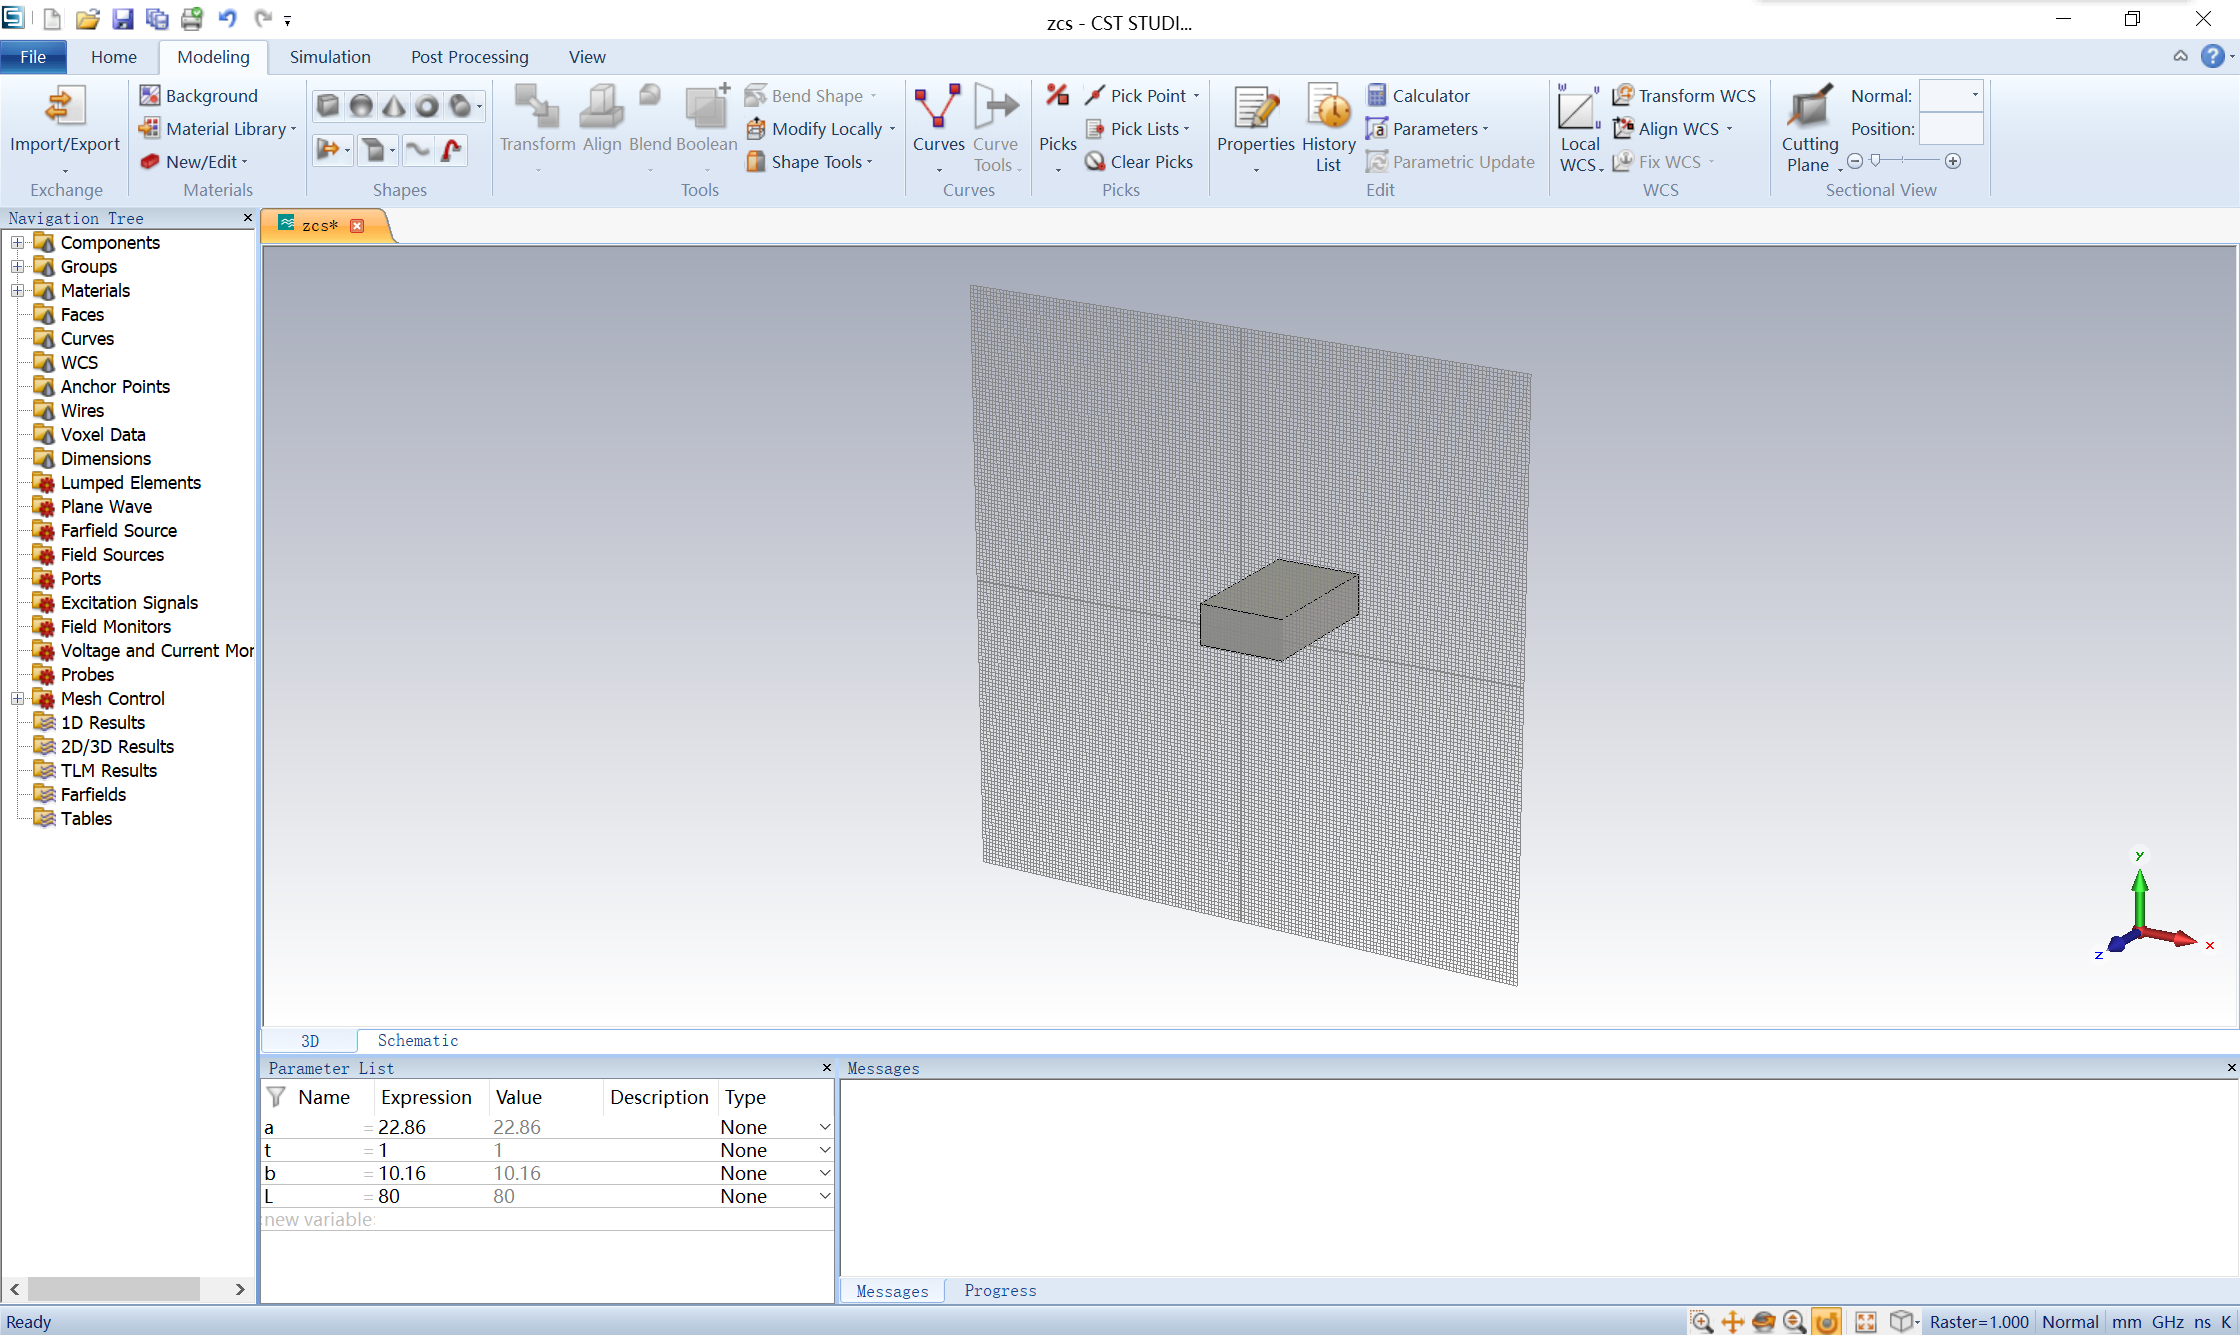
\includegraphics[width = 0.8\textwidth]{figure/创建矩形.png}
            \end{figure}
            \subsubsection{喇叭口径面}
            \begin{figure}[thp]
                \centering
                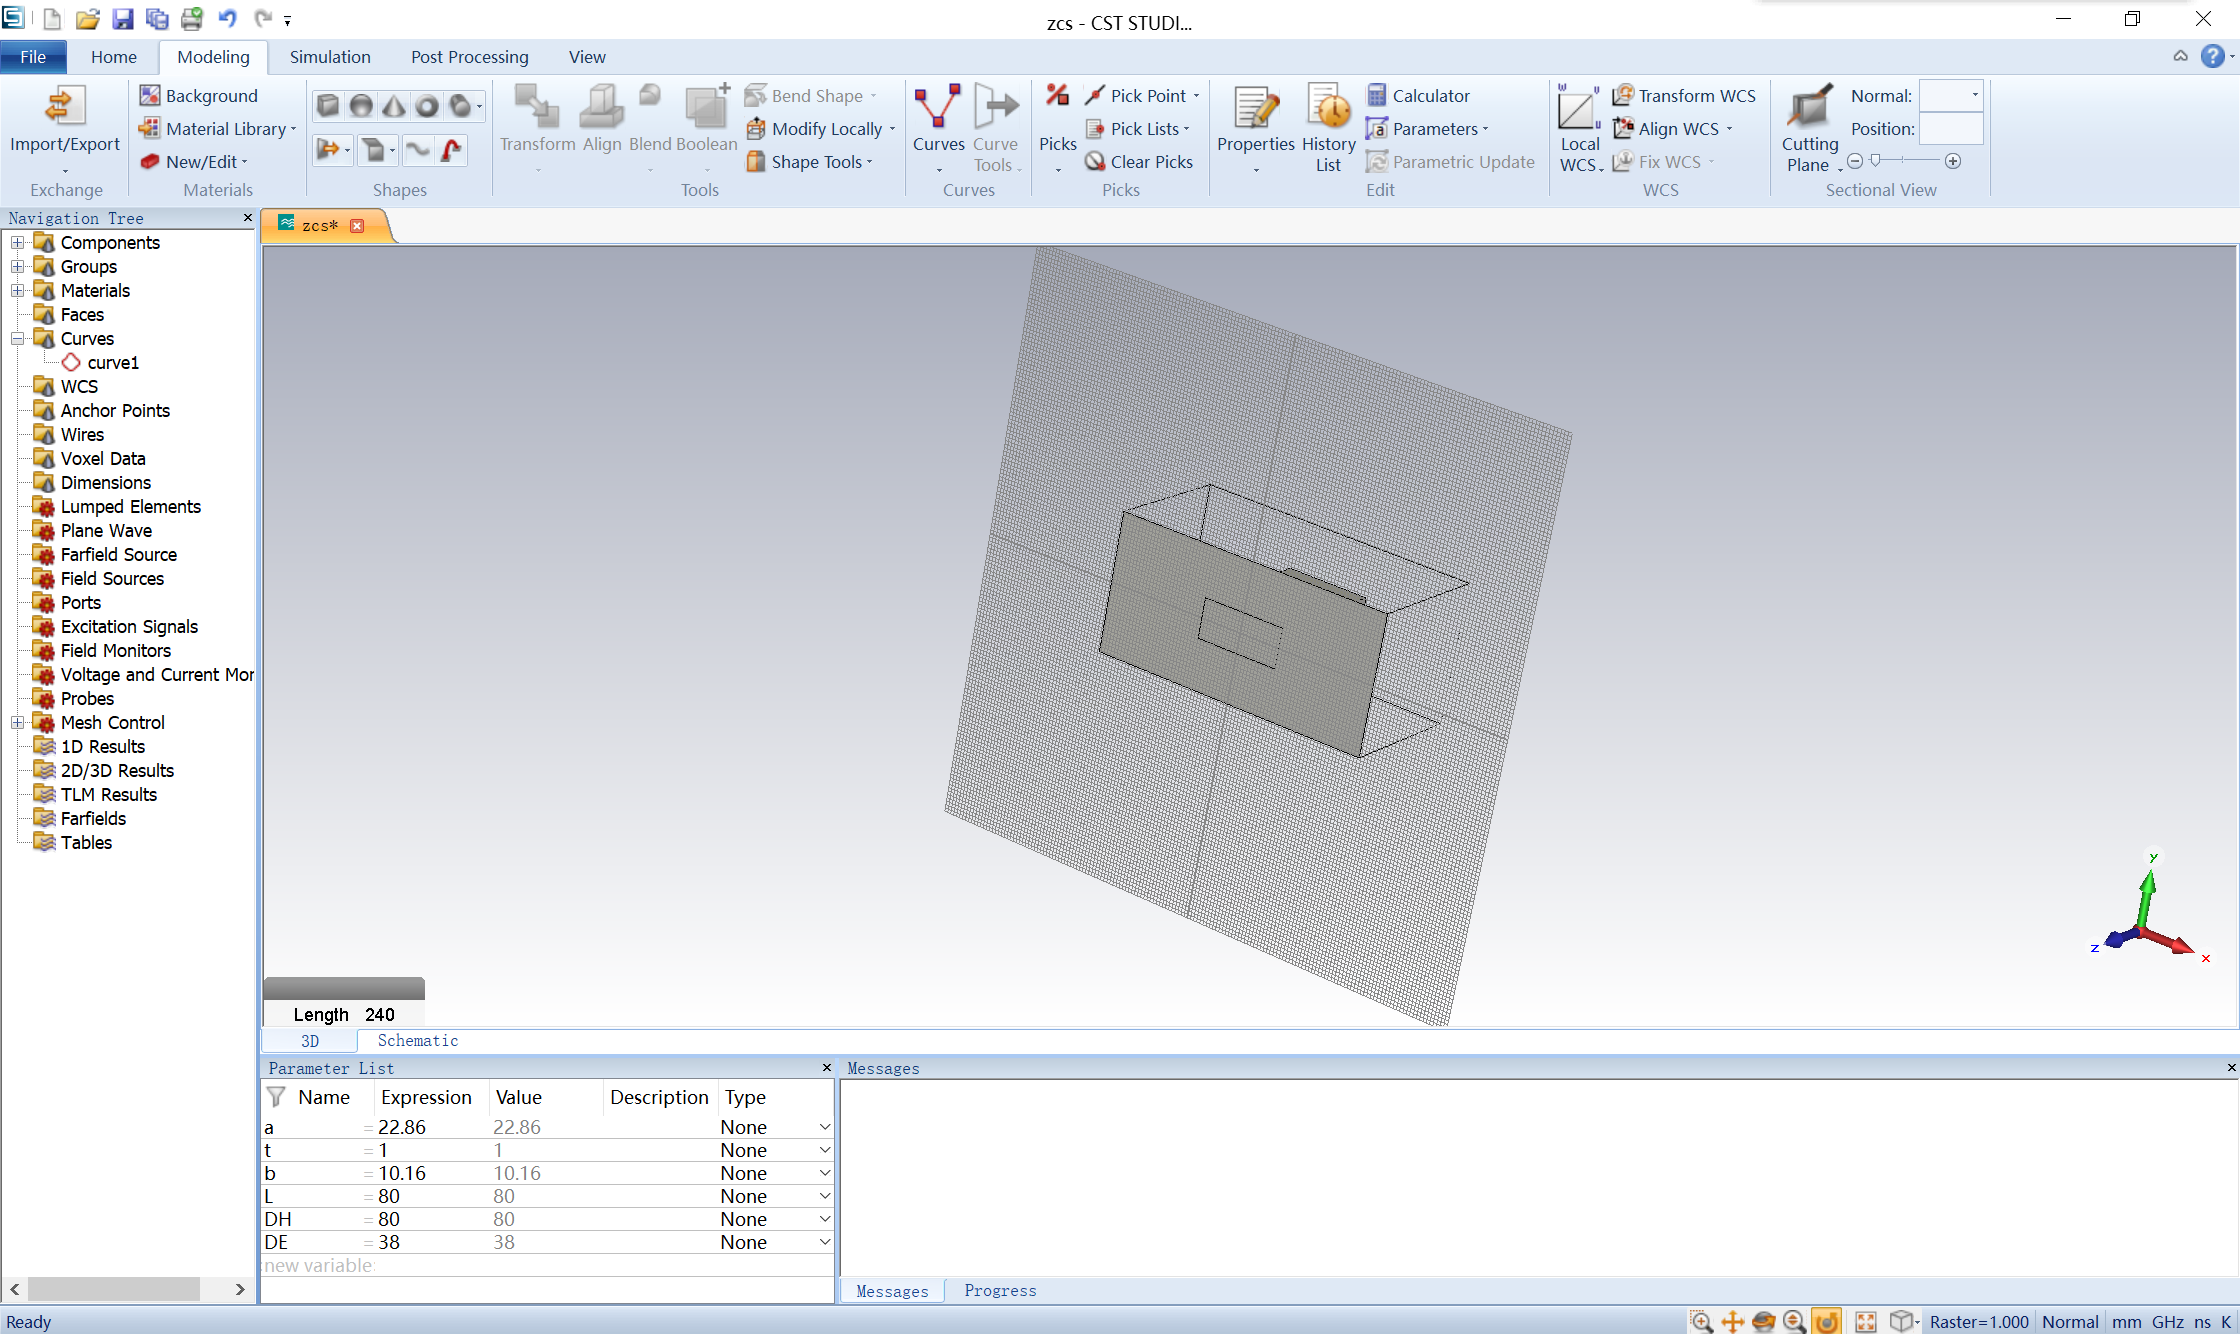
\includegraphics[width = 0.8\textwidth]{figure/创建面.png}
            \end{figure}
            \newpage
            \subsubsection{设置喇叭口径面空间位置}
            \begin{figure}[thp]
                \centering
                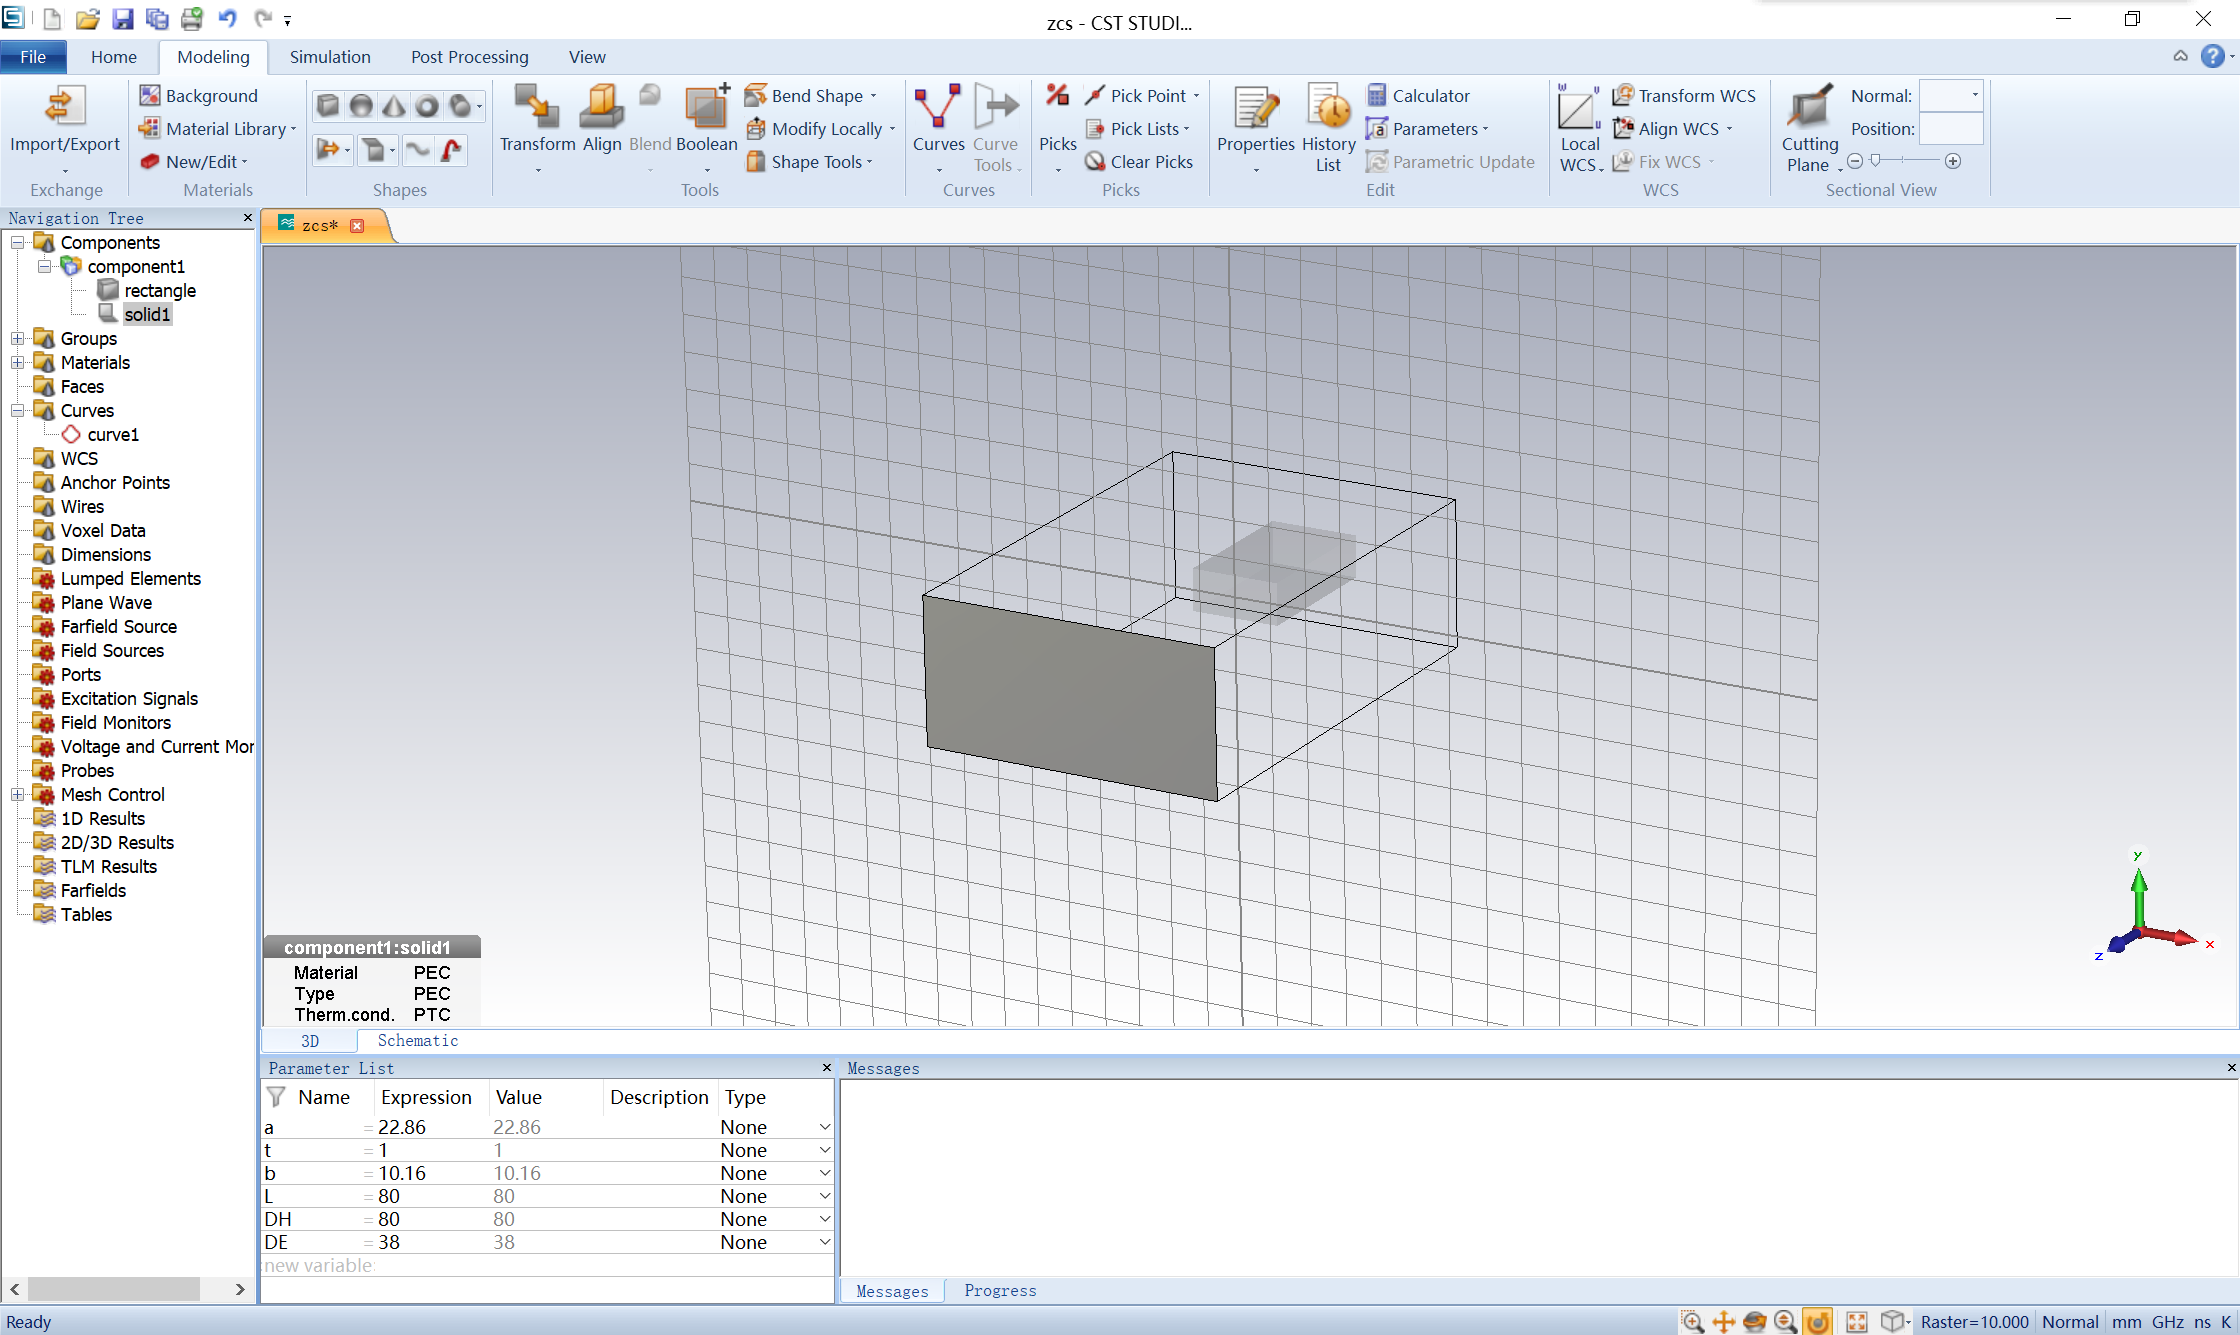
\includegraphics[width = 0.8\textwidth]{figure/平移后.png}
            \end{figure}
            \subsubsection{生成侧壁}
            \begin{figure}[thp]
                \centering
                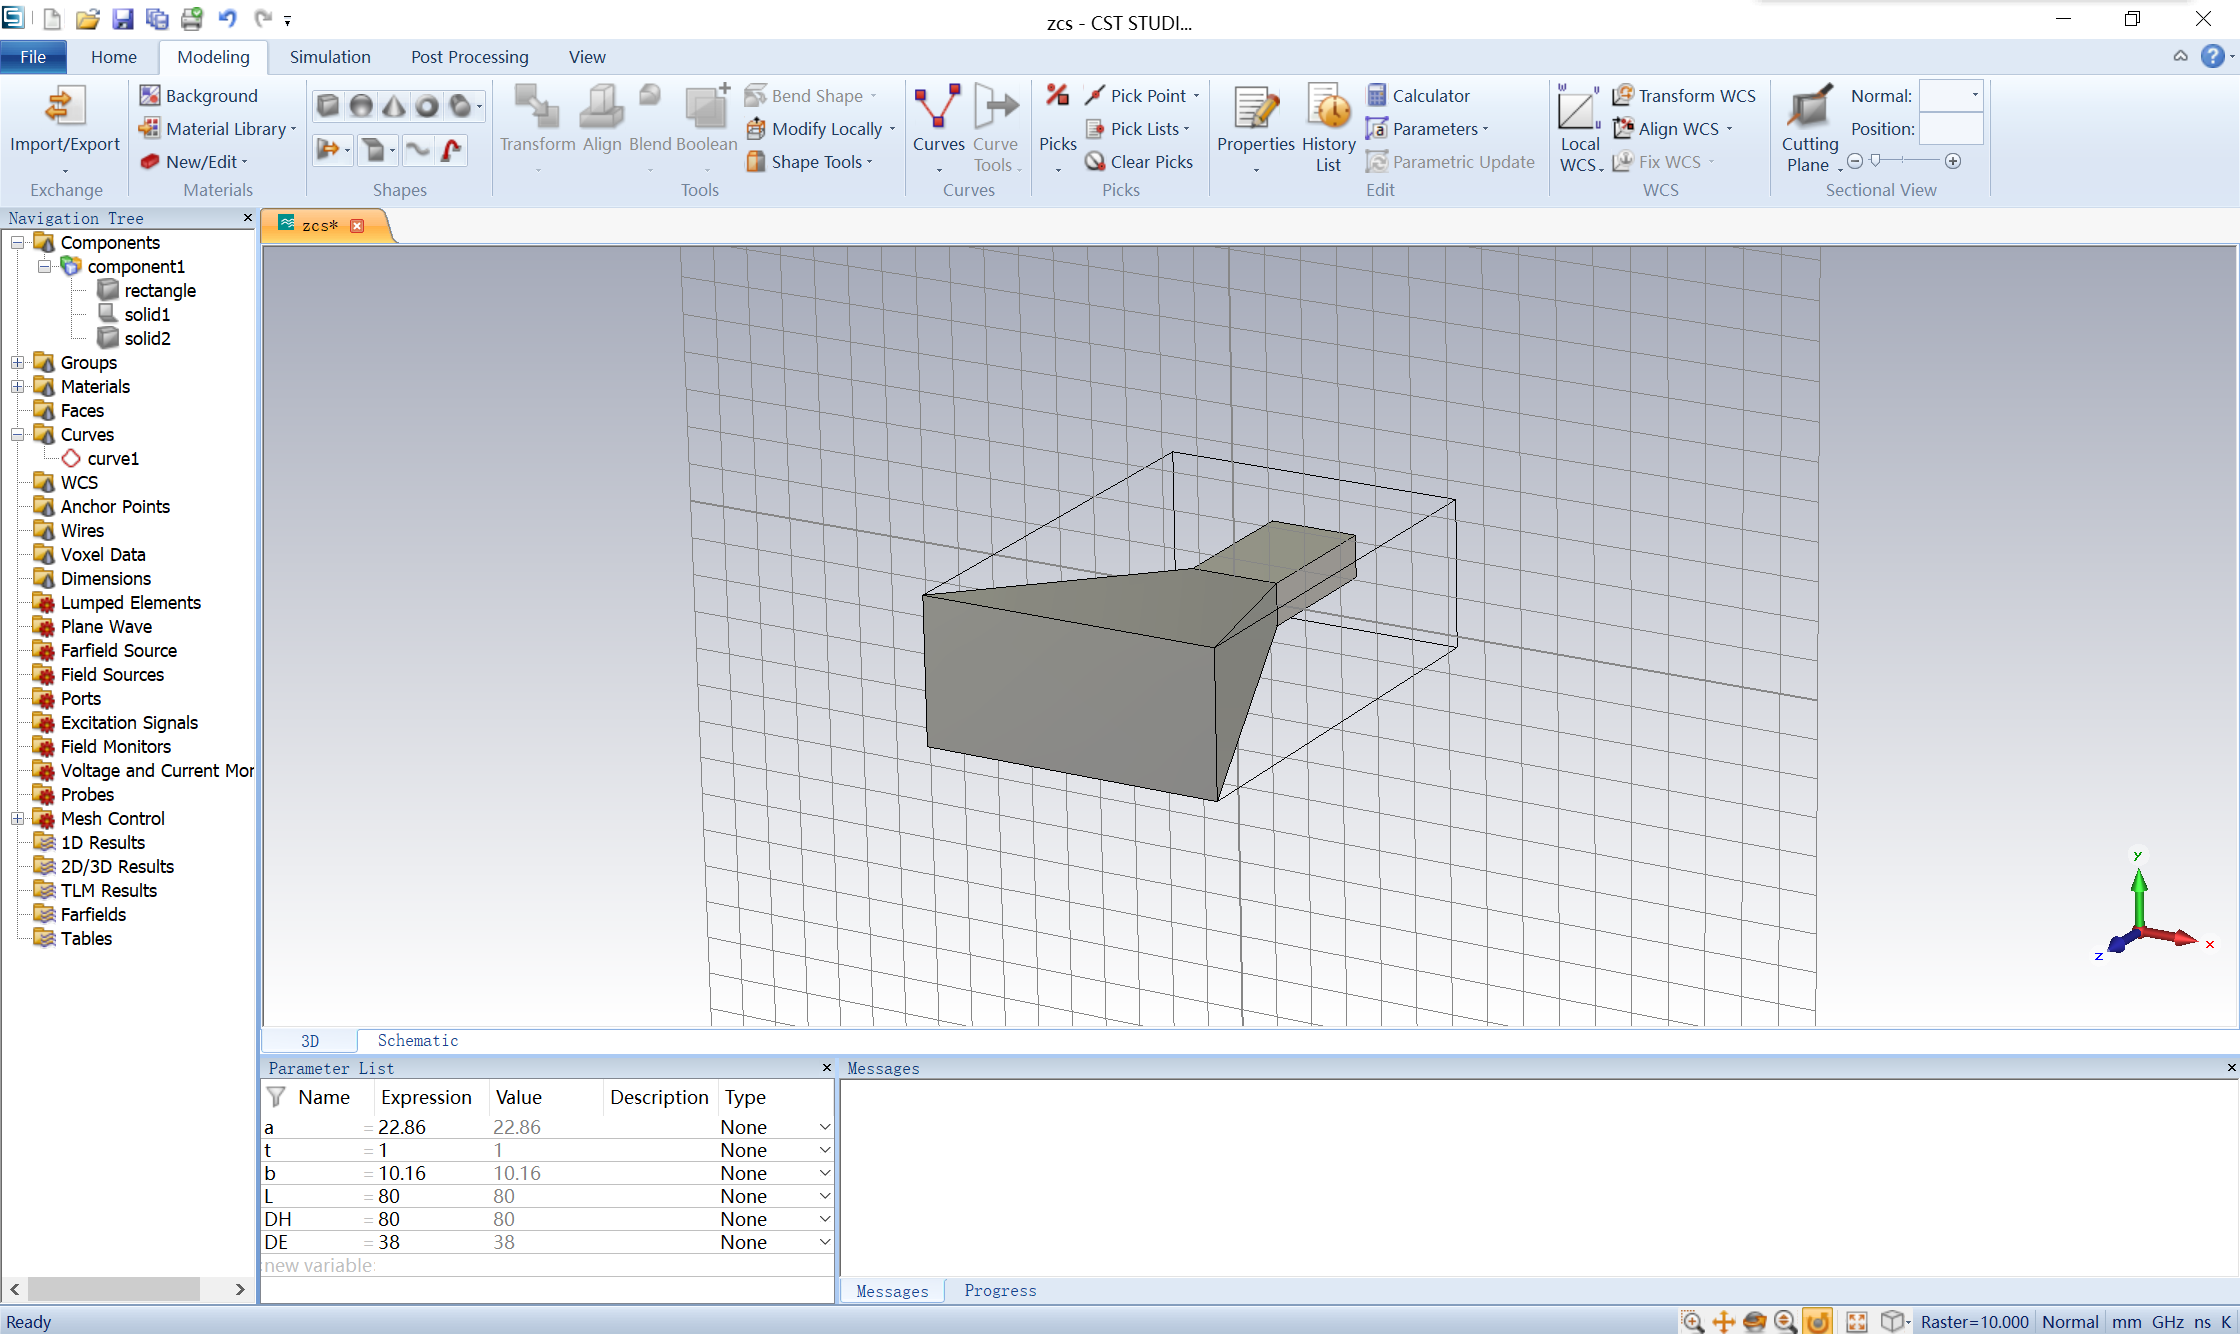
\includegraphics[width = 0.8\textwidth]{figure/喇叭外观.png}
            \end{figure}
            \newpage
            \subsubsection{生成侧壁}
            \begin{figure}[thp]
                \centering
                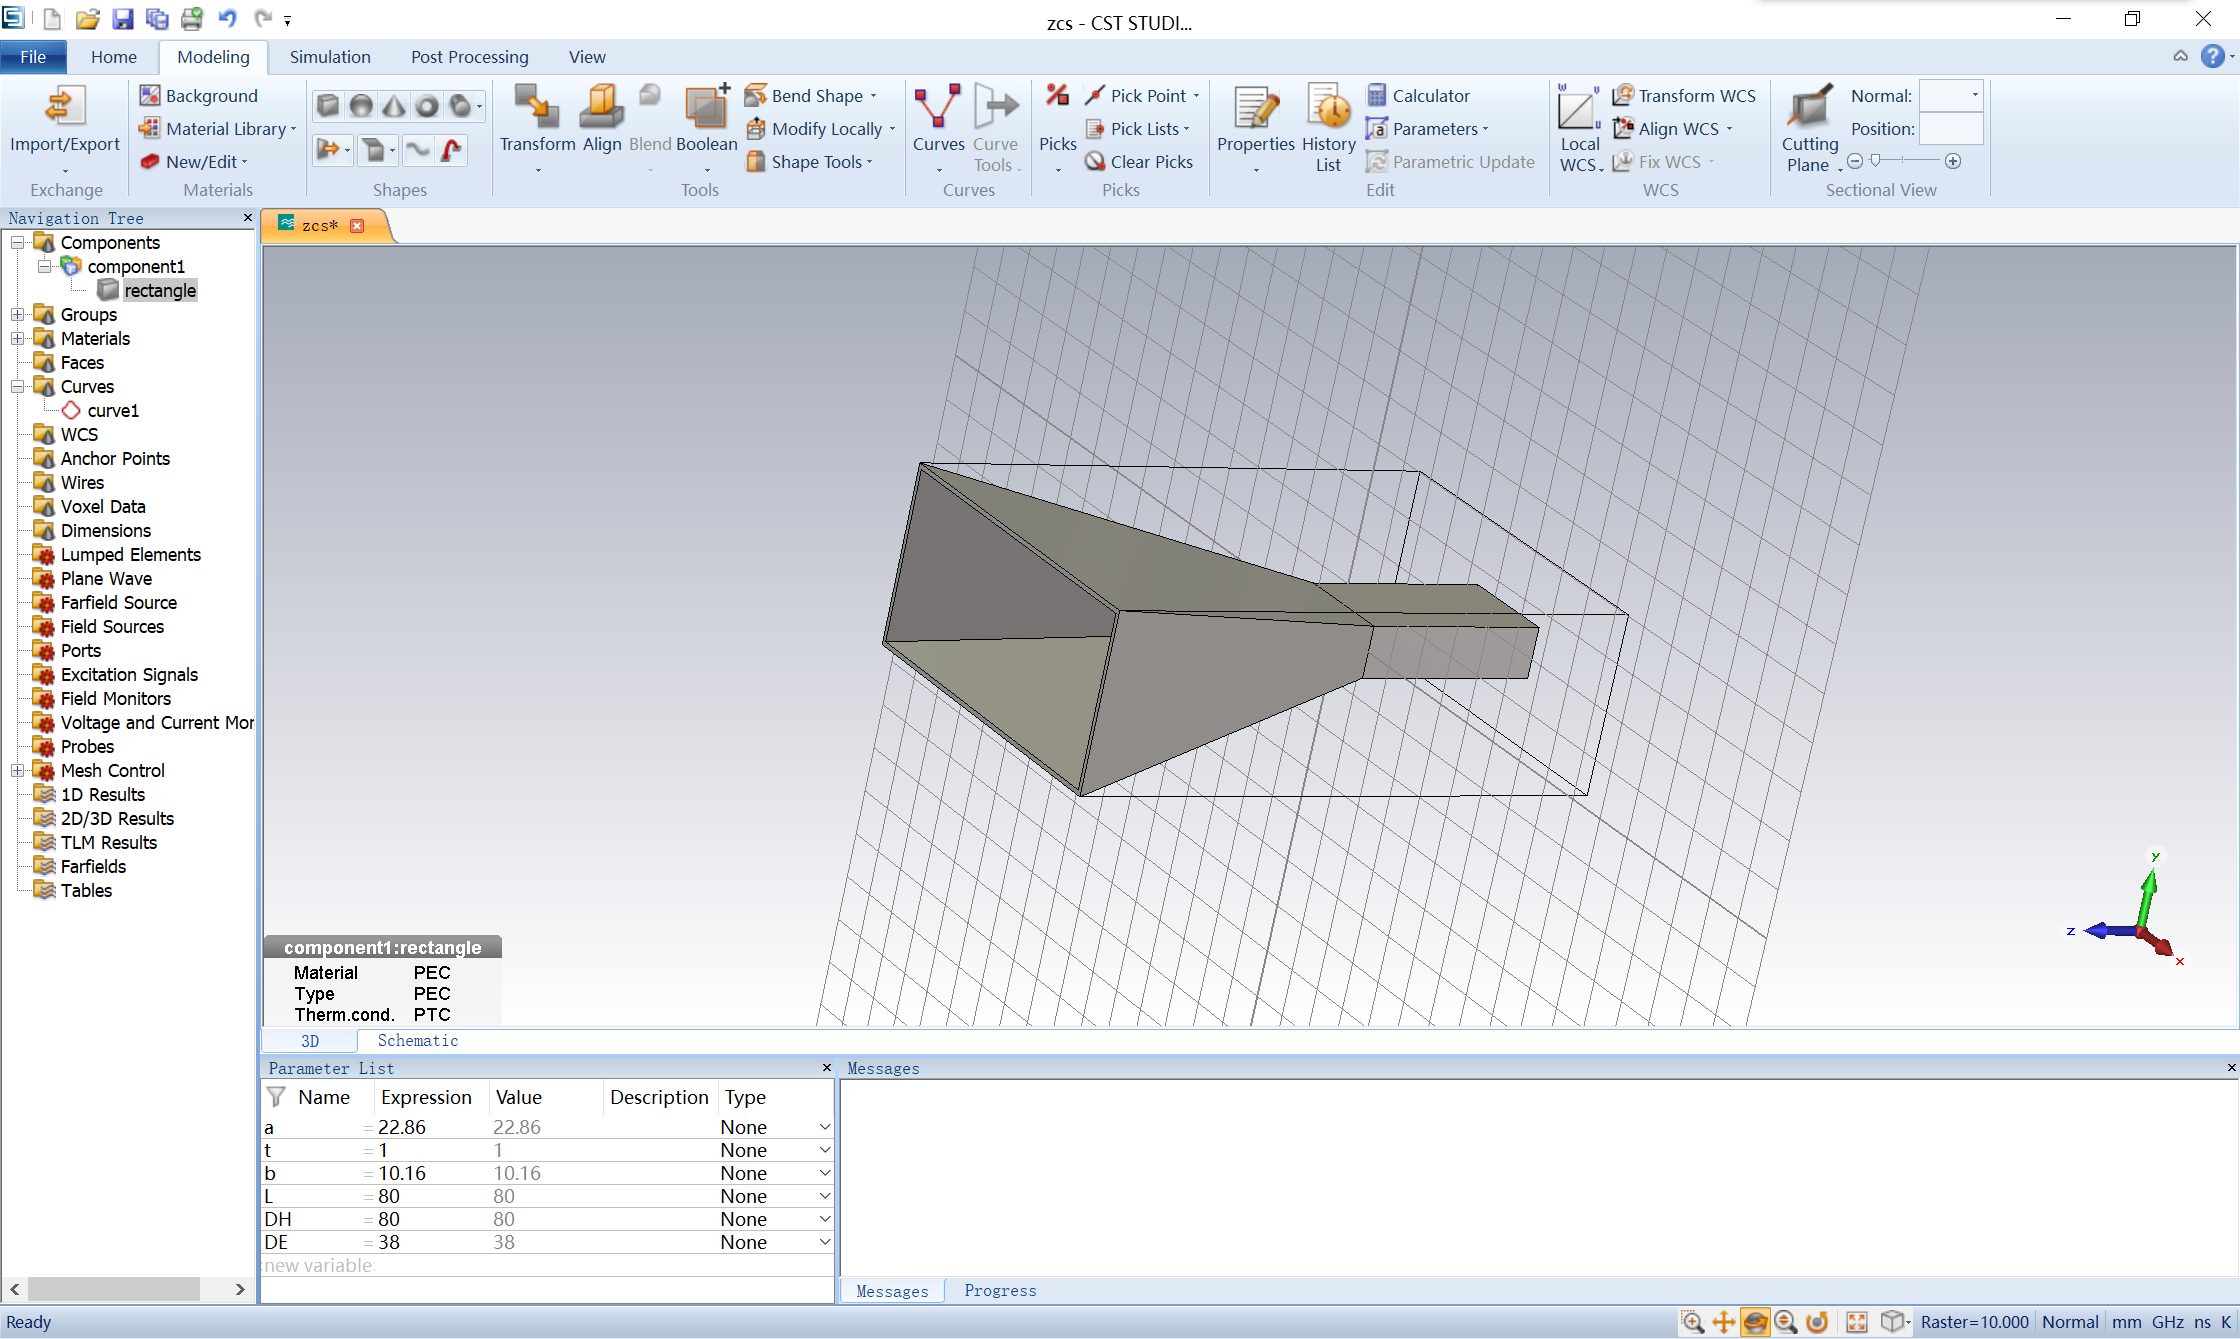
\includegraphics[width = 0.8\textwidth]{figure/掏空后.png}
            \end{figure}

            至此,喇叭模型创建完成,下面进行仿真参数设定

        \subsection{仿真设置}
            \subsubsection{仿真频率设置}
            \begin{figure}[thp]
                \centering
                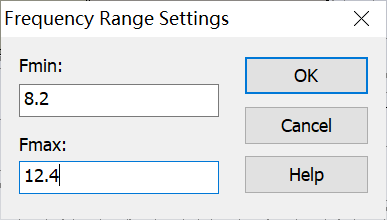
\includegraphics[]{figure/仿真频率.png}
            \end{figure}
            \newpage
            \subsubsection{设置背景}
            \begin{figure}[thp]
                \centering
                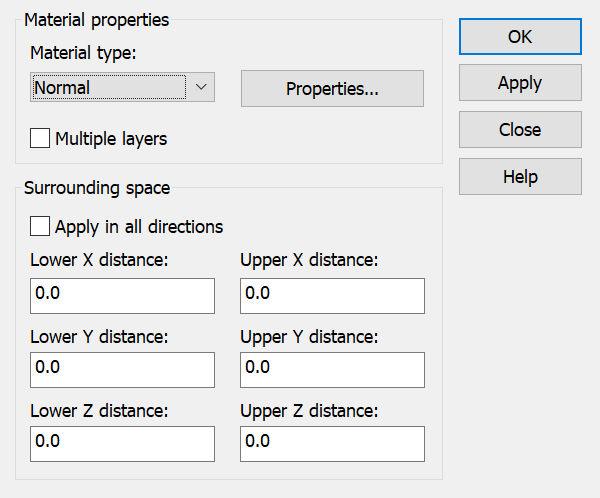
\includegraphics[]{figure/背景设置.png}
            \end{figure}
            \subsubsection{设置边界}
            \begin{figure}[thp]
                \centering
                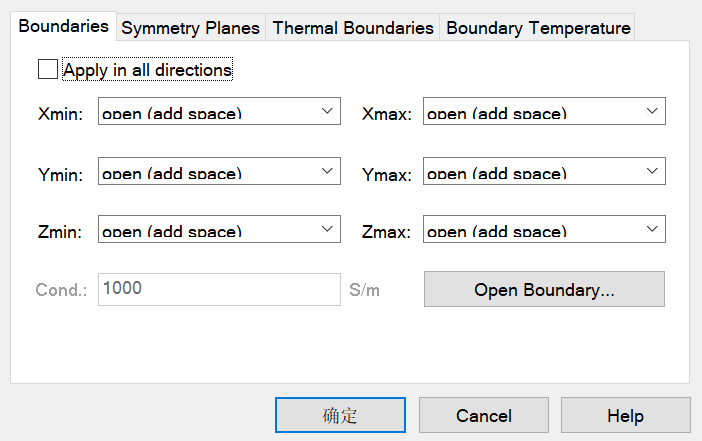
\includegraphics[]{figure/设置边界.png}
            \end{figure}
            \newpage
            \subsubsection{端口设置}
            \begin{figure}[thp]
                \centering
                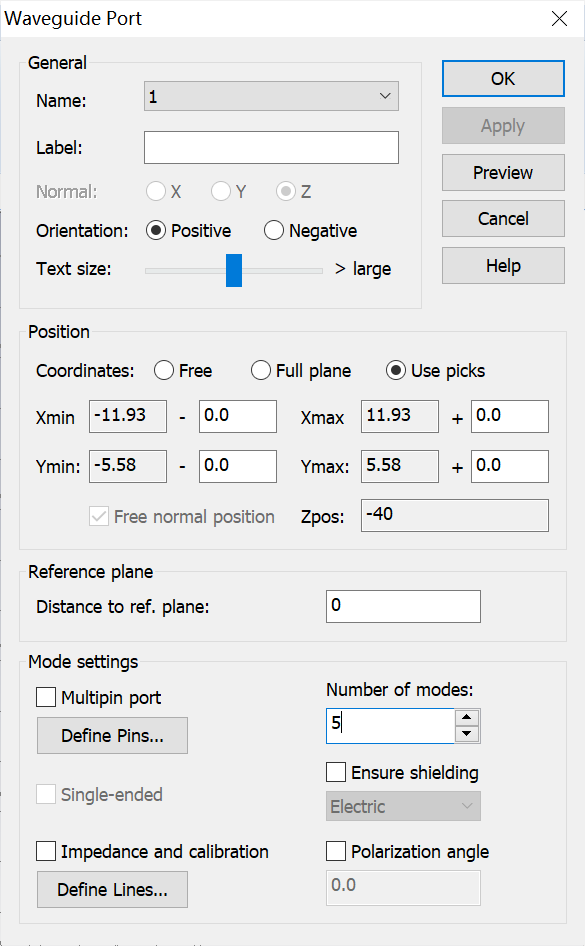
\includegraphics[]{figure/设置端口.png}
            \end{figure}
            \newpage
            \subsubsection{设置监视器}
            \begin{figure}[thp]
                \centering
                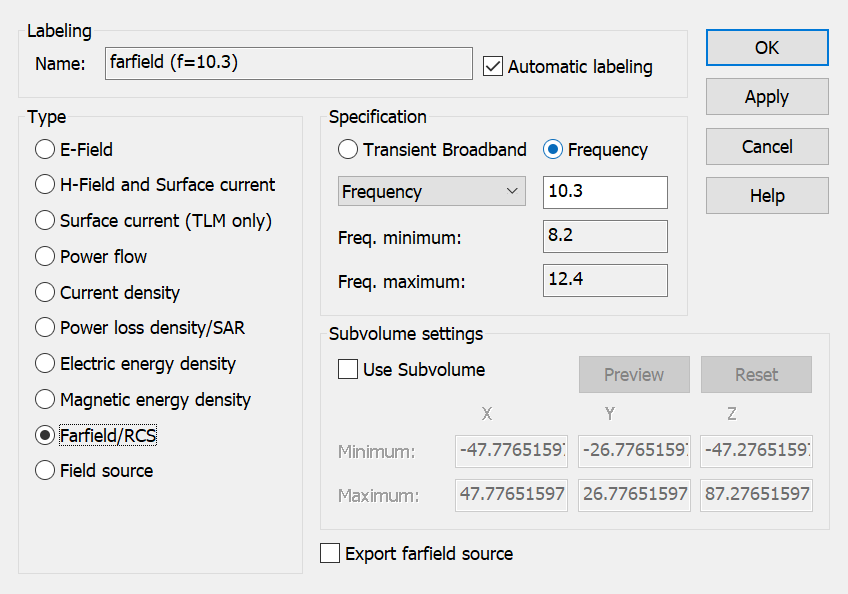
\includegraphics[]{figure/设置监视器.png}
            \end{figure}
        \subsection{模式分析}
            \subsubsection{模式分析设置}
            选中Calculate modes only 选中此选项,只计算端口模式不执行整个时域仿真,可预先了解模式分布,结果如下:
            \begin{figure}[htp]
                \centering
                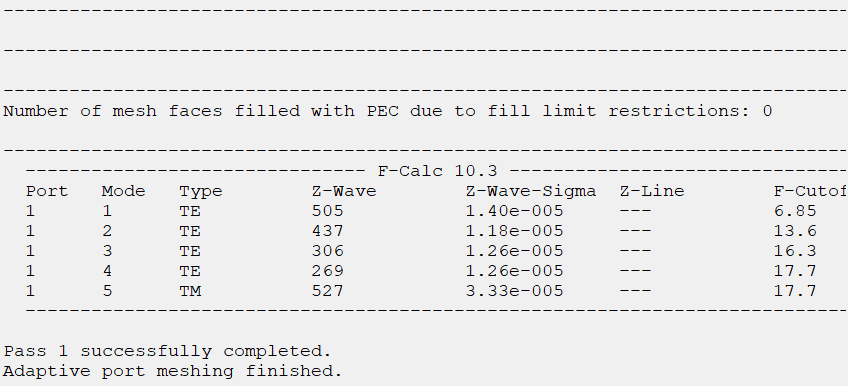
\includegraphics[width = 0.8\textwidth]{figure/端口分析结果.png}
            \end{figure}

            可见仅有mode1在频率范围内,所以仿真时仅仿真mode1
            \subsubsection{仿真设置如下}
            \begin{figure}[htp]
                \centering
                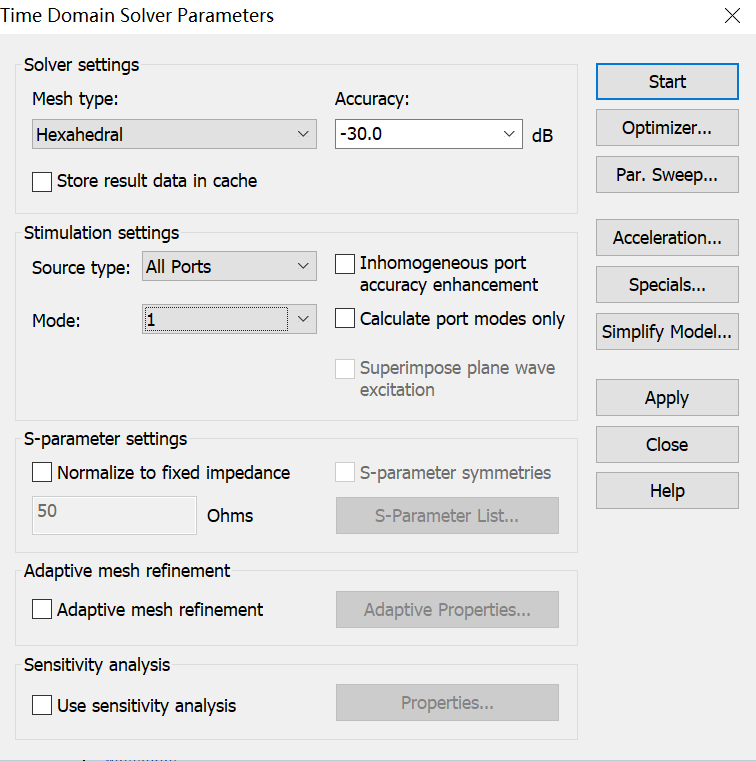
\includegraphics[width = 0.5\textwidth]{figure/仿真设置.png}
            \end{figure}

        \subsection{仿真结果}
            \subsubsection{1D Results}
            在1D Results 中11 S 和驻波曲线
            \begin{figure}[htp]
                \centering
                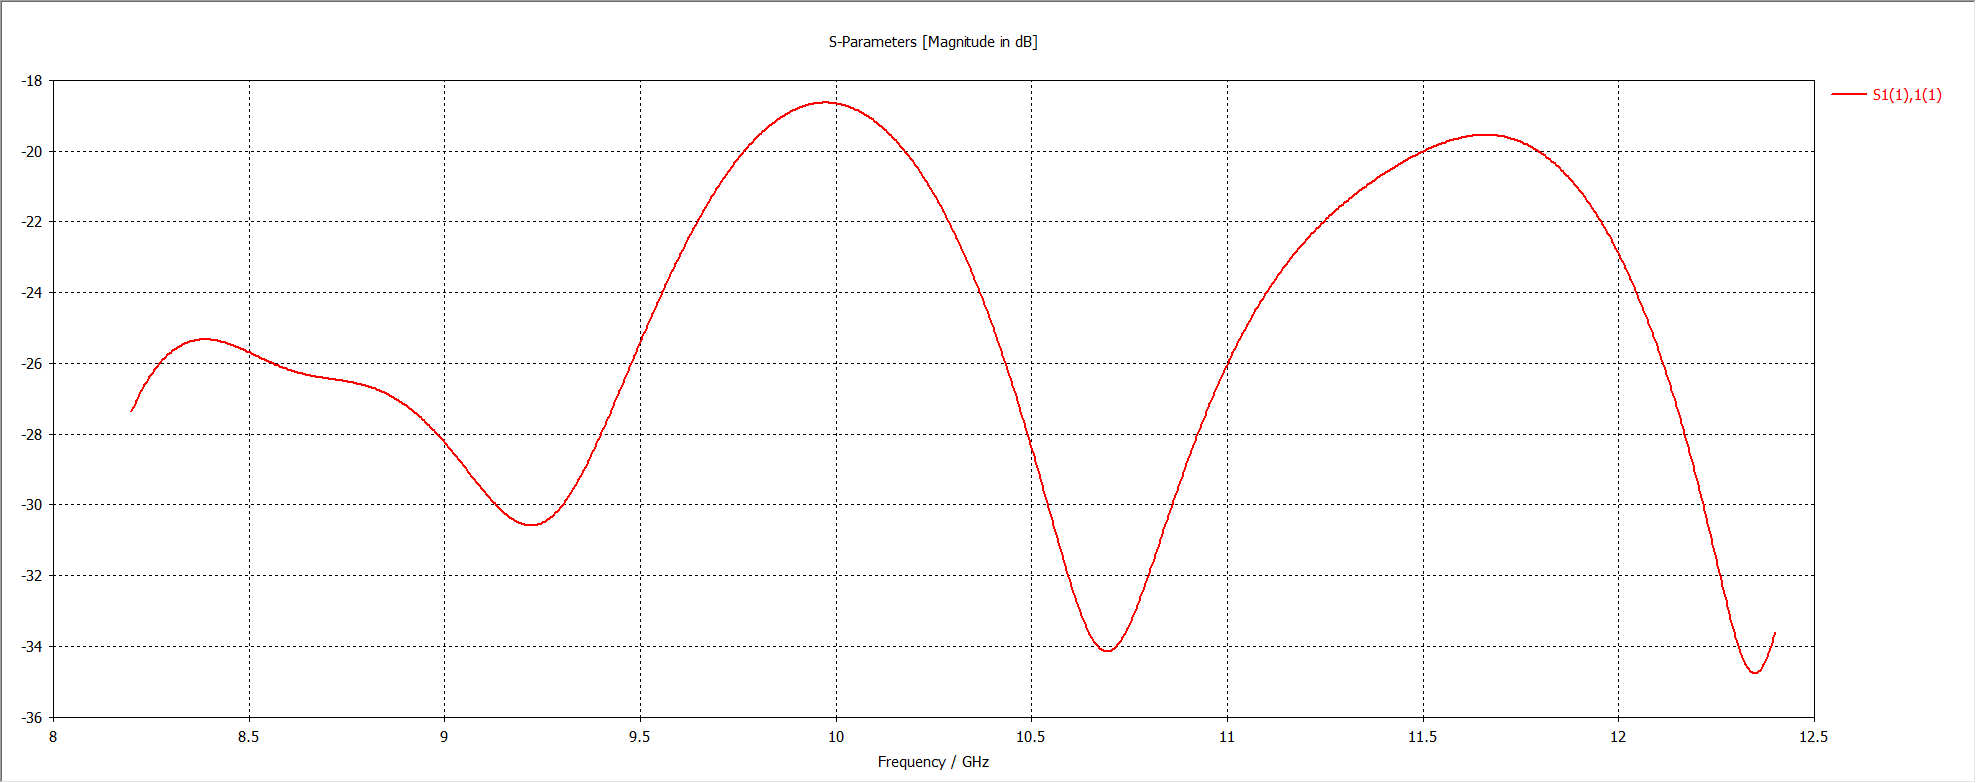
\includegraphics[width = 0.6\textwidth]{figure/s11.png}
            \end{figure}
            \begin{figure}[htp]
                \centering
                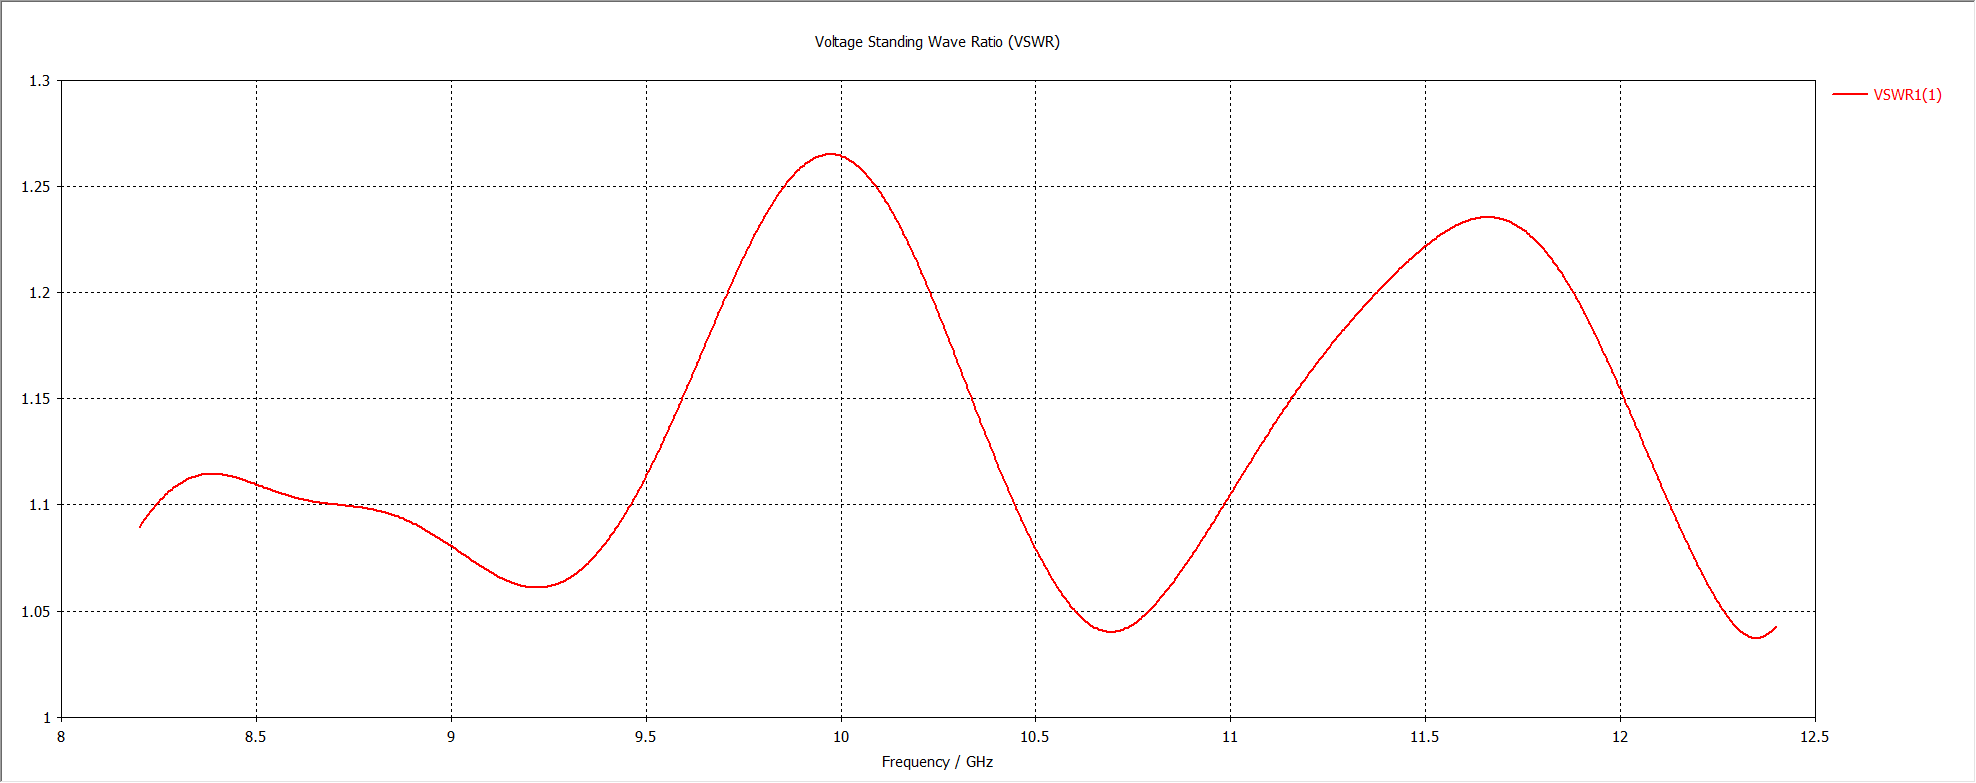
\includegraphics[width = 0.6\textwidth]{figure/驻波比.png}
            \end{figure}
            \subsubsection{方向图}
            \begin{figure}[htp]
                \centering
                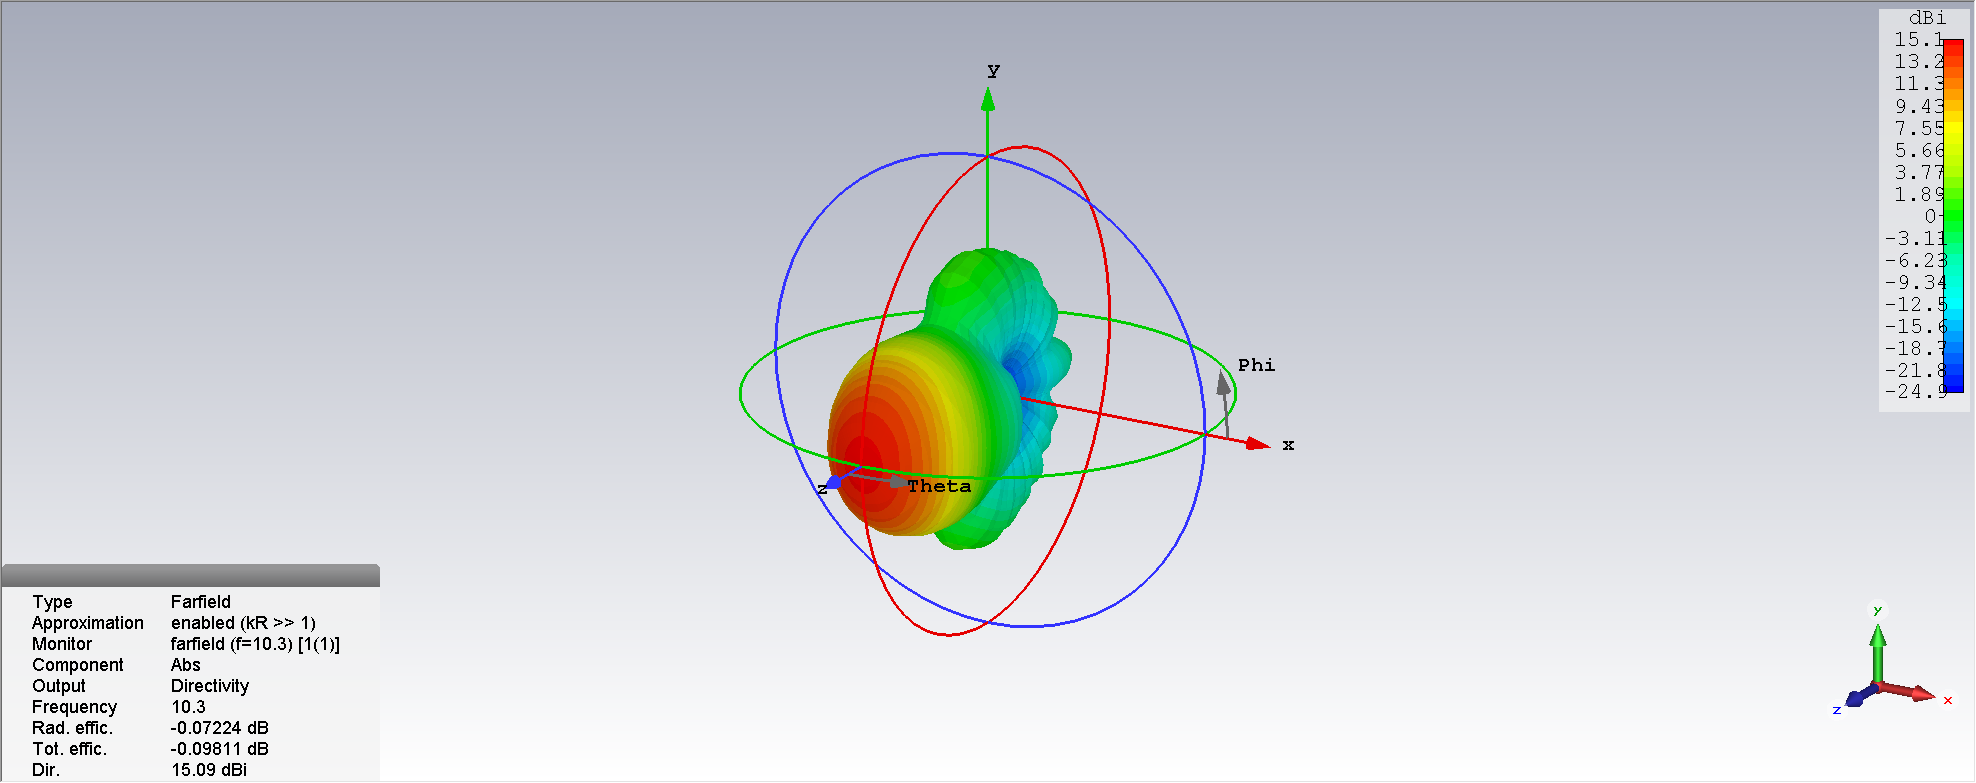
\includegraphics[width = 0.7\textwidth]{figure/3D方向图.png}
            \end{figure}
            \begin{figure}[htp]
                \centering
                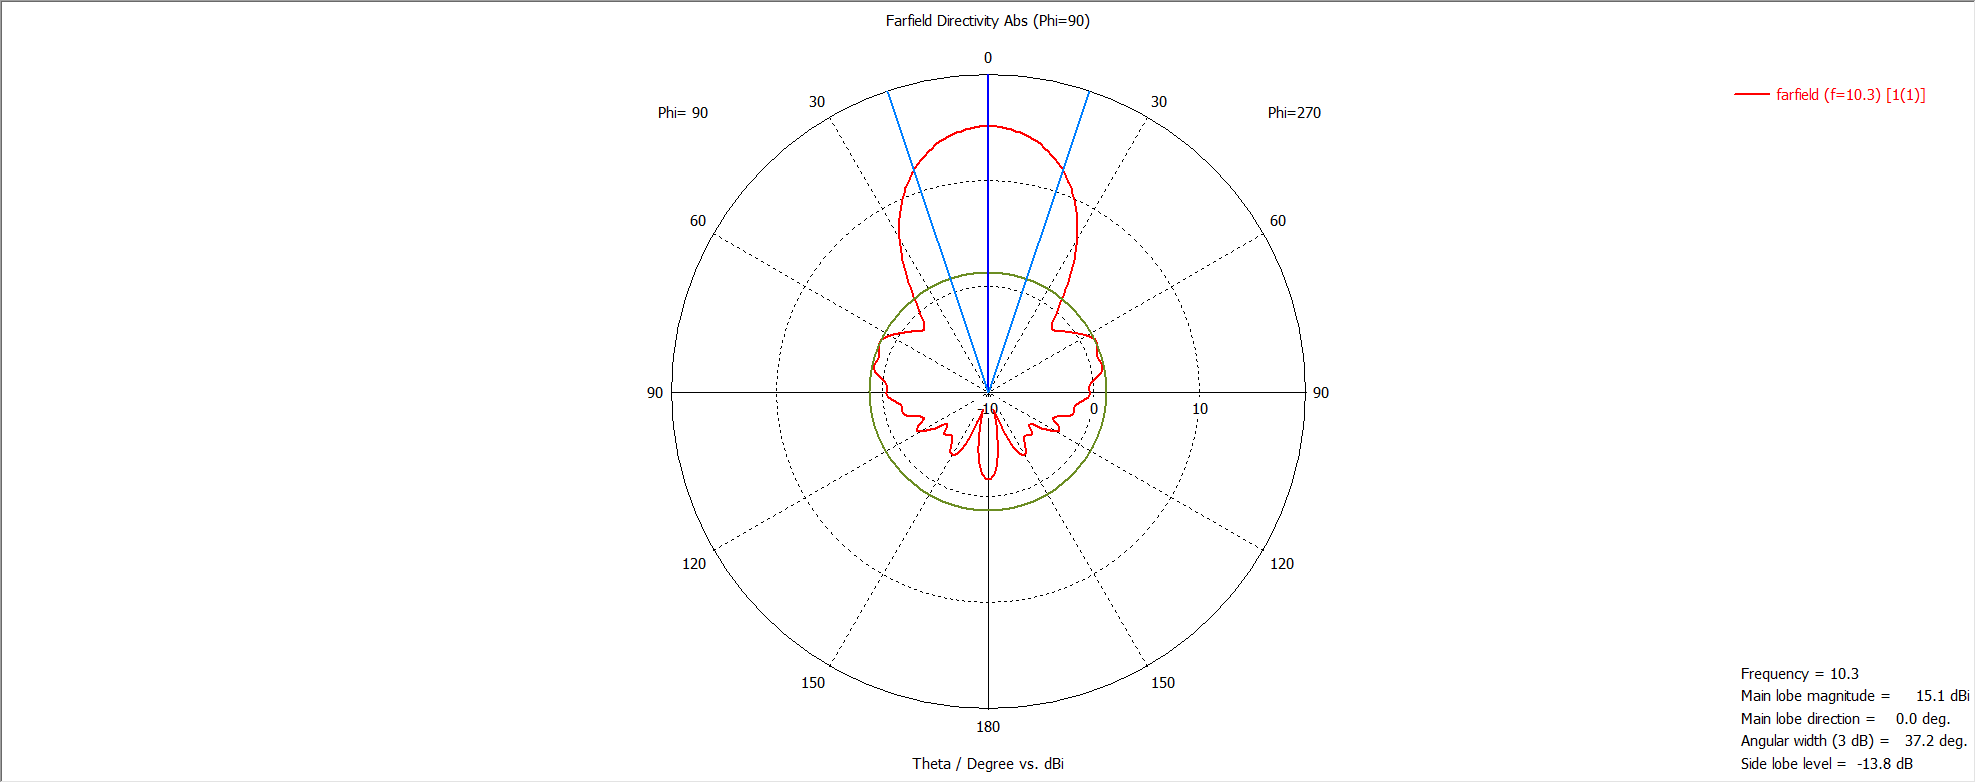
\includegraphics[width = 0.7\textwidth]{figure/polar.png}
            \end{figure}
            \subsubsection{增益}
            \begin{figure}[htp]
                \centering
                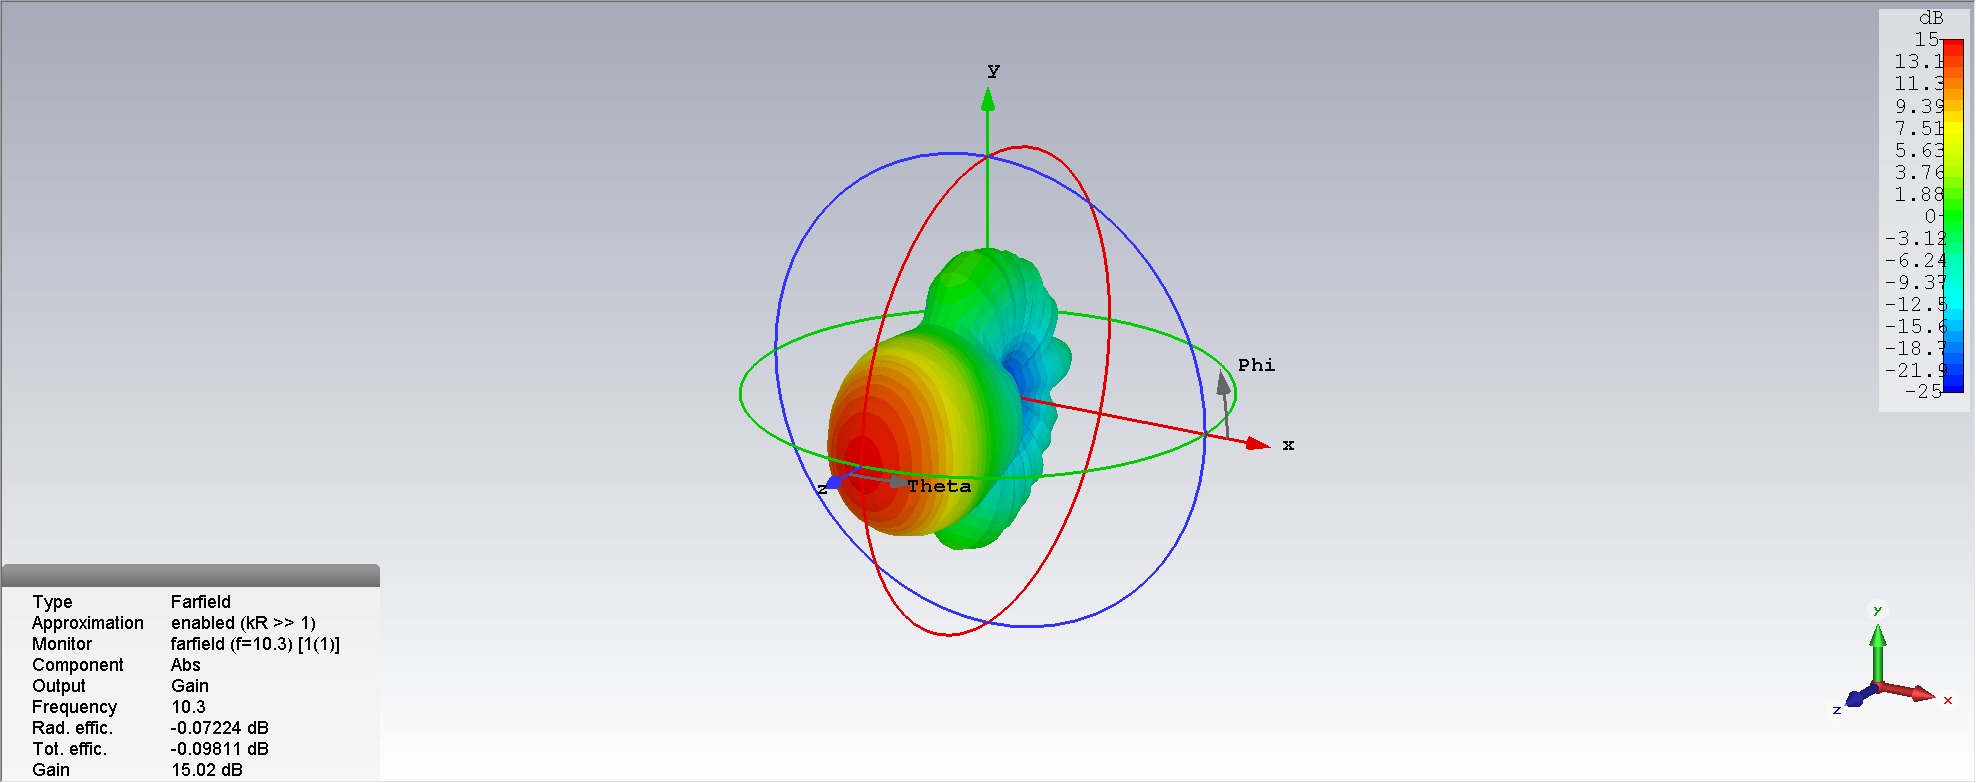
\includegraphics[width = 0.7\textwidth]{figure/Gain3D.png}
            \end{figure}
            \newpage
            \begin{figure}[htp]
                \centering
                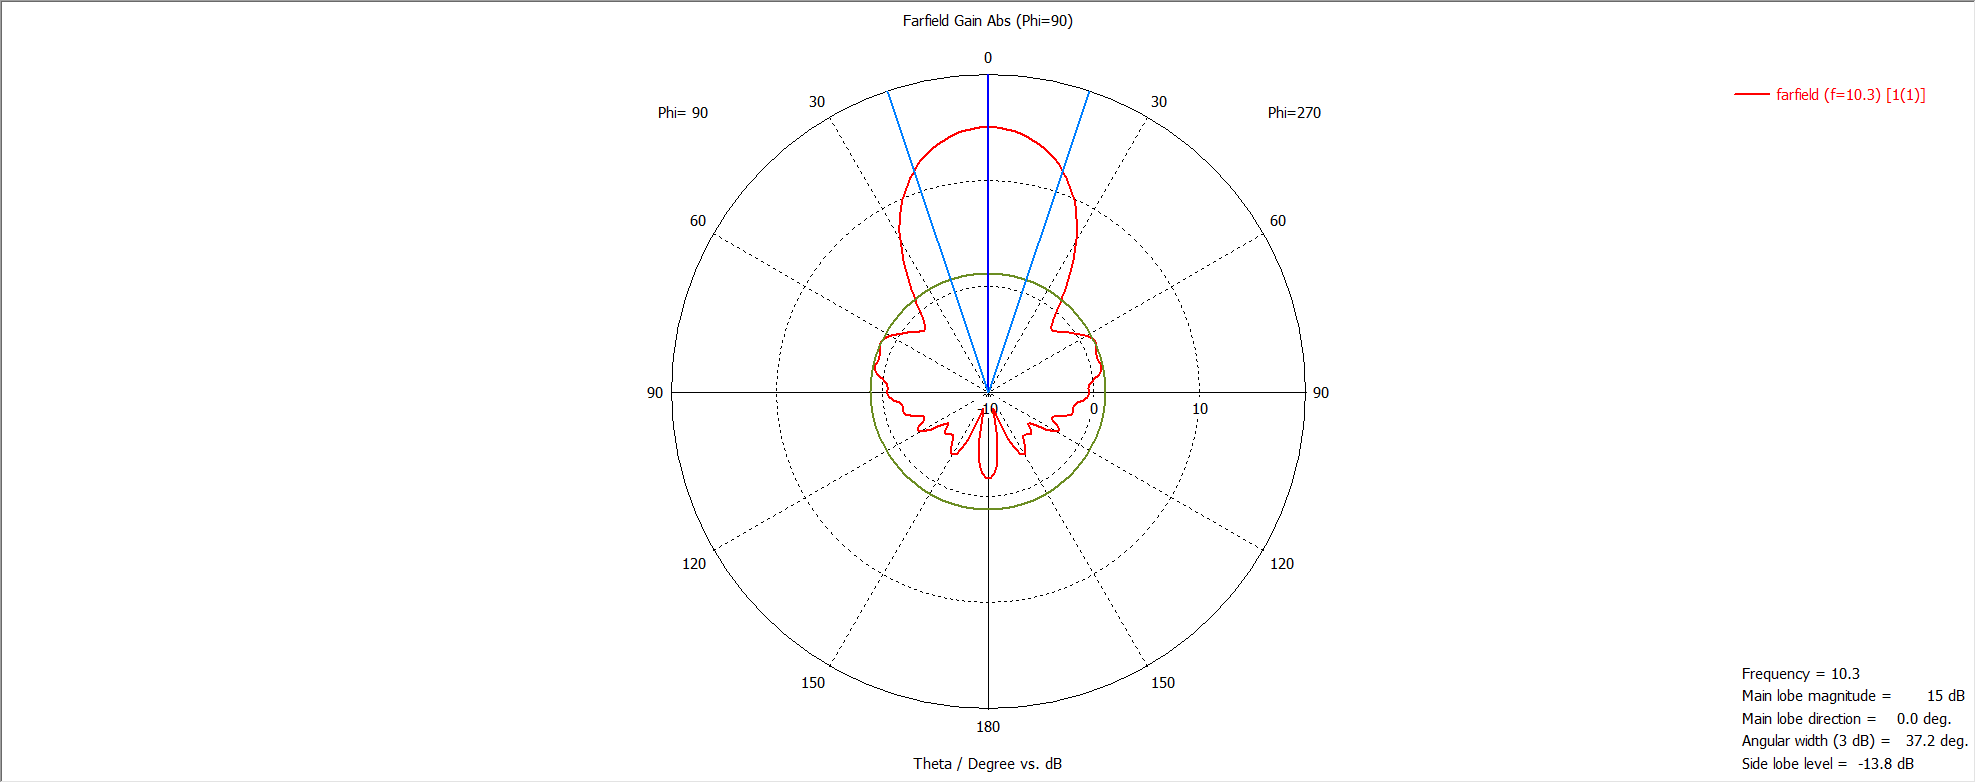
\includegraphics[width = 0.7\textwidth]{figure/Gainpolar.png}
            \end{figure}
            \subsubsection{表面电流}
            \begin{figure}[htp]
                \centering
                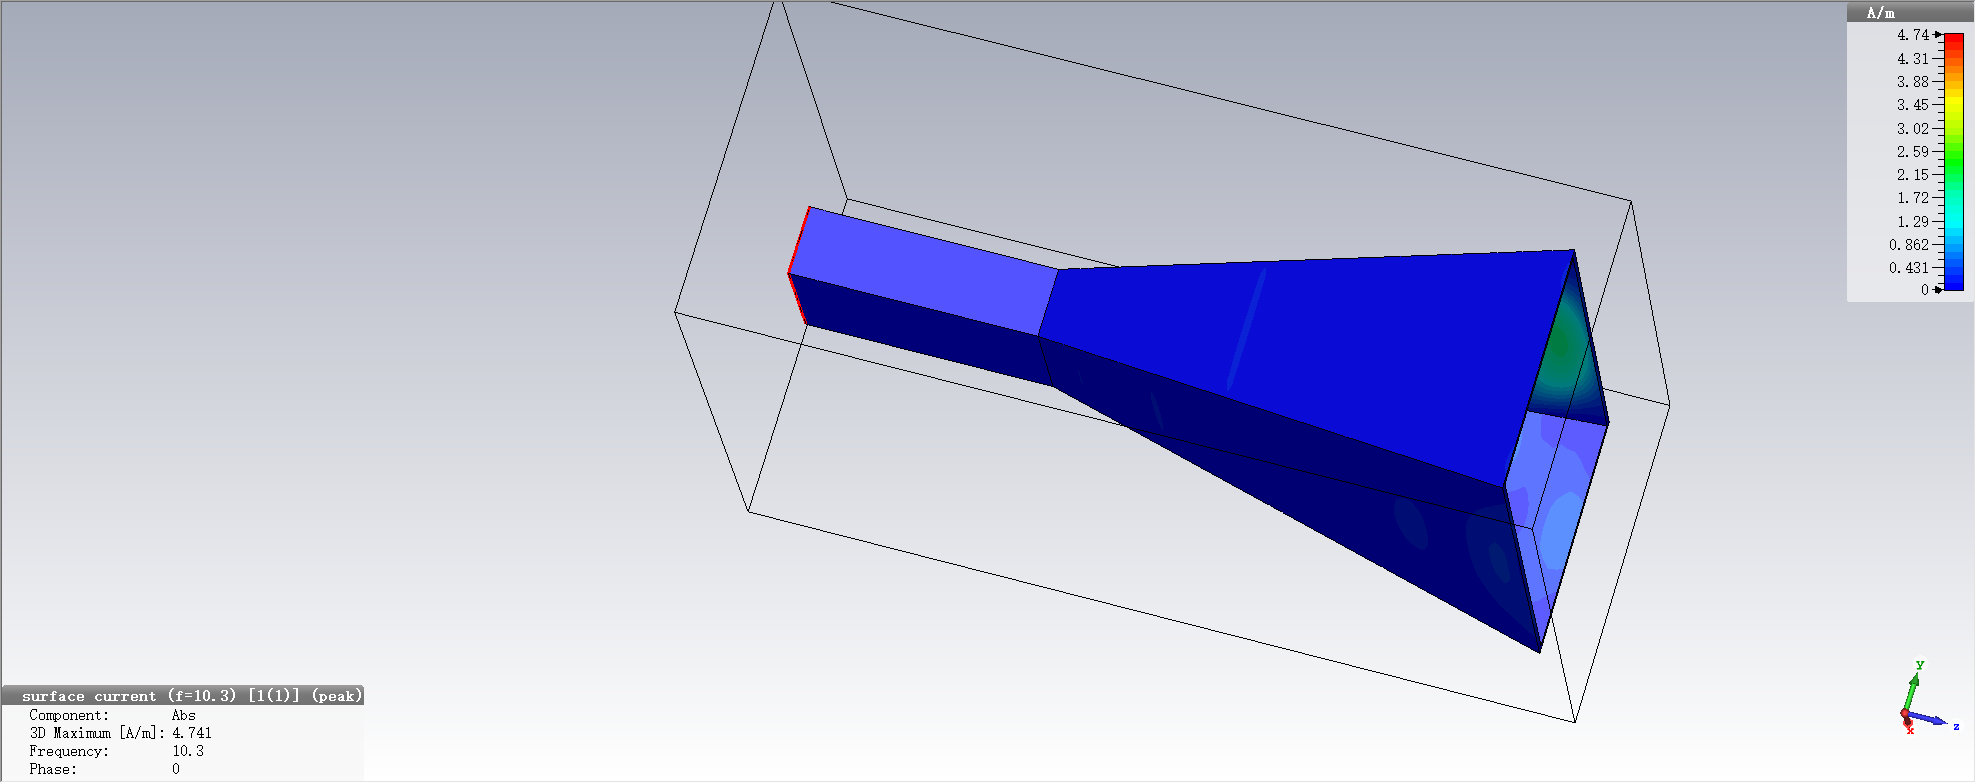
\includegraphics[width = 0.7\textwidth]{figure/表面电流.png}
            \end{figure}
    \section{实验结果分析}
    从仿真结果来看,该矩形波导馈电的角锥喇叭天线的主瓣方向为$\varphi = 0° , \theta  = 0°$ 主瓣宽度为37.2°,主瓣的最大增益为15dB,最大增益的仿真值与理论估计值相近。同时,该天线输入端口的反射系数在工作频段内均在20dB以下,能够较好的工作。

    \section{讨论与心得}
    通过本次实验,我学会了如何利用CST软件进行天线仿真,虽然步骤大多是按照老师给的文档进行的,操作不大熟练,但通过对实验过程以及实验结果的分析,也学到了不少关于天线的知识。例如如何阅读并理解天线的方向图等等。我相信,通过后续天线测量实验的进程,一定更加深刻地掌握天线的相关知识与设计方法。

    \part{喇叭天线辐射特性测量}
    \section{实验目的}
    揭示喇叭天线的幅射特性。

    覆盖的基本概念:
    \begin{enumerate}
        \item 天线辐射方向图
        \item 波束宽度
        \item 天线的极化特性
        \item 电磁波在空间传播中与距离的关系
    \end{enumerate}

    \section{实验原理}
    当今社会尽管人们不一定知道无线寻呼、蜂窝电话、卫星通信、无线广播与电视的具体工作原理,但它们已成为人们生活不可缺少的一部分。在这些无线通信系统中不管是发送还是接收,天线都是一个不可缺省的部件。描述天线的参量很多,择其主要的有:天线方向性、辐射方向图、波束宽度、旁瓣电平、工作频率与响应、效率等等。除此之外,天线发射(或接收)的电磁波都具有极化特性,所谓极化是指电磁波电场矢量的方向,所以接收机接收到的信号大小跟收、发天线的安装方向有关(以下简称发射天线的极化方向或接收天线的极化方向)。如果发射天线所发射电磁波的极化方向与接收天线的极化方向一致时,接收信号最大,若两者正交,接收机将接收不到信号。

    本实验用3公分波段(8-12GHz)喇叭天线揭示天线方向性、波束宽度、波的极化特性。

    实验装置如图2-29,装置包括三部分:分别是信号发射端、接收端和天线移动架。发射端由固态振荡源、微波衰减器、小喇叭天线连接组成,并装在一个旋转云台上。发射端喇叭天线可以绕矩形波导轴向旋转,由此可以改变发射电磁波的极化方向,其极化角度可从指示刻度盘读出;发射功率的大小可用微波衰减器来调节。云台可在垂直面和水平面上转动,用于测量发射天线的方向性特性;发射端还装有一个可移动的金属栅网;天线移动架可以使发射端沿着移动架轨道平移,从而改变收、发喇叭天线之间的距离,其测量值可以从移动架上的刻度尺读取。接收端将喇叭天线与微波晶体检波器连接在一起固定不动

    用到的方程为:
    $$P_r = \frac{P_tG_tG_r\lambda^2}{\left( 4\pi R \right)^2}\left( W \right)$$
    其中R为收、发天线间距离。

    最佳角锥喇叭天线增益: 
    $$G = 0.51\frac{4\pi A_p}{\lambda^2}$$
    $A_p$为喇叭口的面积

    喇叭天线半功率波束宽度:
    H面:$2\theta _{0.5}\approx 1.18\frac{\lambda}{D_H}\left( rad \right)$

    E面:$2\theta _{0.5}\approx 0.89\frac{\lambda}{D_E}\left( rad \right)$

    远区场条件:$R\gg \frac{2D_HD_E}{\lambda}$

    \section{实验数据}
    \newpage
    \subsection{天线距离与接收功率}
    \begin{table}[H]
        \centering
        \begin{tabular}{|c|c|c|}
        \hline
            距离R(m) & 实际测量值(dB) & 相对归一化功率 \\ \hline
            1.0 & -30 & 1 \\ \hline
            1.1 & -31.2 & 0.759 \\ \hline
            1.2 & -32.6 & 0.550 \\ \hline
            1.3 & -33.4 & 0.457 \\ \hline
            1.4 & -34.2 & 0.380 \\ \hline
        \end{tabular}
        \caption{天线距离与接收功率关系}
    \end{table}

    
    

        \subsection{极化测量}
        \subsubsection{天线极化测量}
        \begin{table}[H]
            \centering
            \begin{tabular}{|l|l|l|}
            \hline
                发射喇叭天线角度$\theta$ & 实际测量值(dB) & 相对归一化功率 \\ \hline
                0 & -30 & 1 \\ \hline
                10 & -30.4 & 0.912 \\ \hline
                20 & -31.1 & 0.776 \\ \hline
                30 & -32.8 & 0.525 \\ \hline
                40 & -34.8 & 0.331 \\ \hline
                50 &  -38  & 0.158 \\ \hline
                60 & -42.2 & 0.060 \\ \hline
                70 & -48.5 & 0.014 \\ \hline
                80 & -58.6 & 0.001 \\ \hline
                90 & -65.0 & 0.000 \\ \hline
            \end{tabular}
        \end{table}

        \subsubsection{极化栅网特性测量}
        \begin{table}[H]
            \centering
            \begin{tabular}{|c|c|c|}
            \hline
            极化栅网角度 & 实验测量值 & 相对归一化功率 \\ \hline
            0 & -40 & 1 \\ \hline
            90 & -69 & 0.001 \\ \hline
            45 & -56 & 0.025 \\ \hline
            \end{tabular}
            \caption{极化栅网特性测量数据}
        \end{table}

        \subsection{喇叭天线辐射方向图测量}
        \begin{table}[H]
            \centering
            \resizebox{\textwidth}{!}{
                \begin{tabular}{|c|c|c|c|c|c|c|c|c|c|c|c|c|c|c|c|c|c|c|c|}
                    \hline
                    天线水平方向转角 & -90 & -80 & -70 & -60 & -50 & -40 & -30 & -20 & -10 & 0 & 10 & 20 & 30 & 40 & 50 & 60 & 70 & 80 & 90 \\ \hline
                    实验测量值 & -74.2 & -75 & -75.5 & -70.5 & -63.4 & -57.2 & -51.6 & -46 & -41.8 & -40 & -41 & -45 & -50.6 & -55 & -61.2 & -69 & -77.5 & -73.8 & -76.2 \\ \hline
                    相对归一化功率 & 0.0004 & 0.0003 & 0.0003 & 0.0009 & 0.0046 & 0.0191 & 0.0692 & 0.2512 & 0.6607 & 1 & 0.7943 & 0.3162 & 0.0871 & 0.0316 & 0.0076 & 0.0013 & 0.0002 & 0.0004 & 0.0002 \\ \hline
                \end{tabular}
            }
            \caption{天线水平方向图测试数据}
        \end{table}

        \begin{table}[H]
            \centering
            \resizebox{\textwidth}{!}{
                \begin{tabular}{|c|c|c|c|c|c|c|c|c|c|c|c|c|c|}
                    \hline
                    天线垂直方向转角 & -60 & -50 & -40 & -30 & -20 & -10 & 0 & 10 & 20 & 30 & 40 & 50 & 60 \\ \hline
                    实验测量值 & -79.5 & -70 & -71.8 & -66 & -52.6 & -43.2 & -40 & -42.8 & -53.6 & -64.8 & -68.5 & -76.5 & -73 \\ \hline
                    相对归一化功率 & 0.0001 & 0.001 & 0.0007 & 0.0025 & 0.055 & 0.4786 & 1 & 0.5248 & 0.0437 & 0.0033 & 0.0014 & 0.0002 & 0.0005 \\ \hline
                \end{tabular}
            }
            \caption{天线垂直方向图测量数据}
        \end{table}

        水平面-3dB功率时的波束宽度:25°

    \section{实验结果与分析}
        \subsection{根据测得的数据作出电磁波传播与距离的关系曲线。}
        利用MATLAB对上述数据进行拟合,得到如下拟合结果:
        \begin{figure}[H]
            \centering
            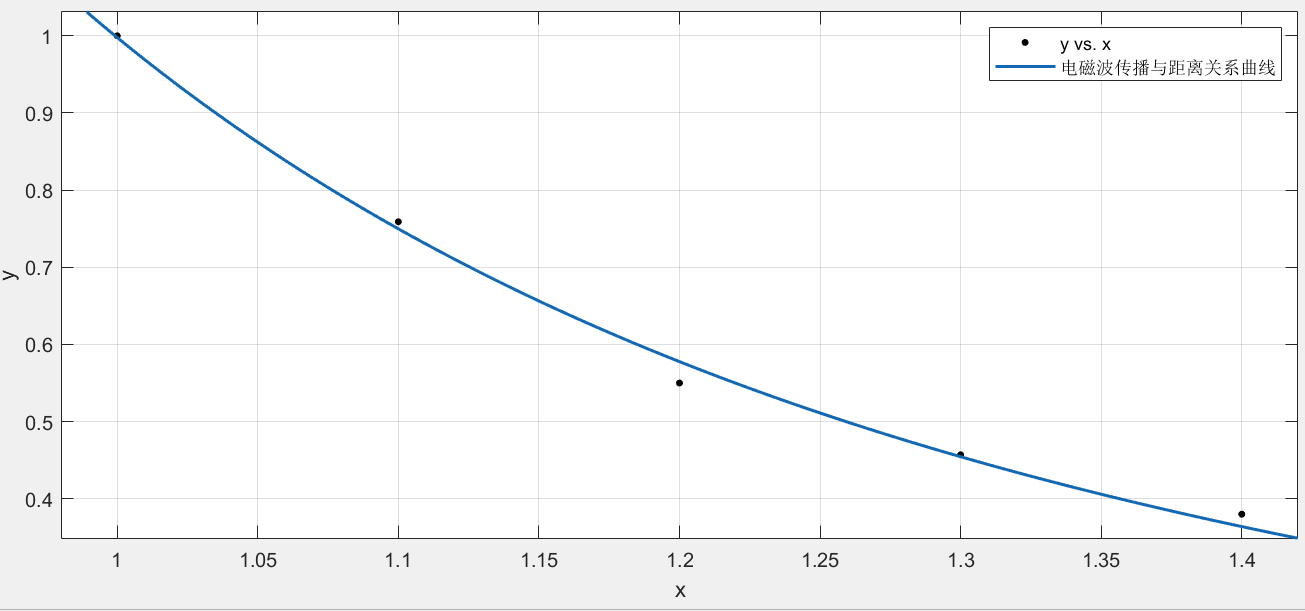
\includegraphics[width = 0.9\textwidth]{figure/电磁波传输与距离关系图.png}
            \caption{拟合曲线}
        \end{figure}

        
        \subsection{所作出的电磁波传播与距离的关系曲线接近$\frac{1}{R}$,$\frac{1}{R^2}$还是$\frac{1}{R^3}$?与理论预期值符合吗?}
    
        \begin{figure}[H]
            \centering
            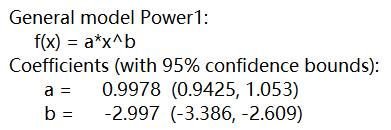
\includegraphics[]{figure/2拟合结果.png}
            \caption{拟合结果}
        \end{figure}

        由上述结果可知,拟合而成的曲线与$\frac{1}{R^3}$比较接近,但是这与理论值中的$\frac{1}{R^2}$并不符合,分析之后我认为是实验室中其他同学的设备以及实验环境中人员过多,走动过于频繁带来了这一误差。

        \subsection{根据数据作出发射喇叭天线极化曲线,横坐标为天线极化角度$\theta$。}
        \begin{figure}[H]
            \centering
            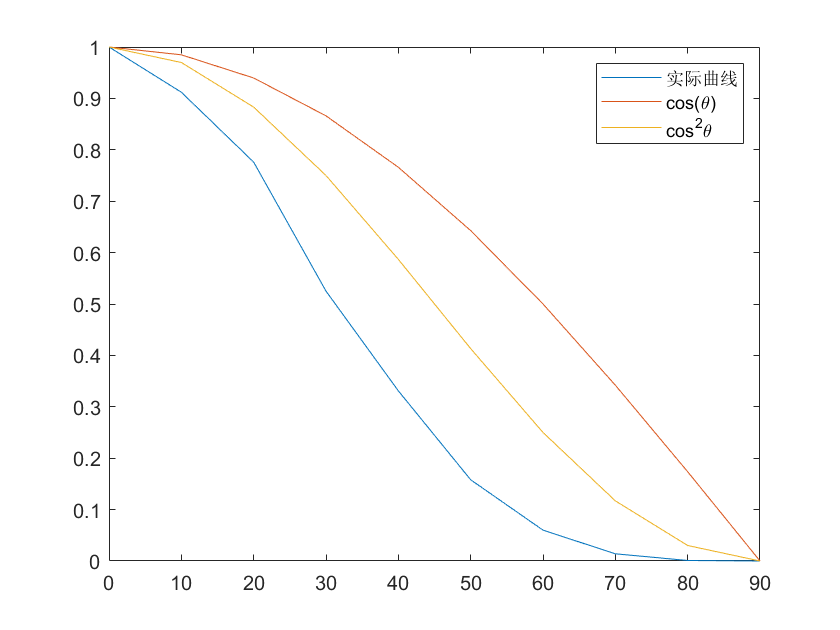
\includegraphics[width = 0.9\textwidth]{figure/天线极化测量.png}
            \caption{天线极化曲线}
        \end{figure}

        \subsection{问题回答}
            \subsubsection{从发射喇叭天线极化特性曲线看,接收喇叭天线所接收到的功率与发射喇叭天线极化角度$\theta$的关系是符合$\cos\theta$还是$\cos^2\theta$关系?}
            由上述曲线可得,接收喇叭天线所收到的功率与发射喇叭天线极化角度$\theta$的关系是符合$\cos^2\theta$。
            \subsubsection{如果发射喇叭天线和接收喇叭天线的极化角相差90°,而极化器相对于发射喇叭天线的极化角度为45°,极化器对系统的影响如何?}
            发射的信号经极化器分解成与极化器平行和垂直的两路信号,在经过接收喇叭,原始信号的一半被收到

        \subsection{对发射天线计算远区场距离(工作频率9.375GHz),实验中是否符合远区场条件?}
        $\because 2D_ED_H/\lambda = 0.1896m , R = 1.2m$
        $\therefore $符合远区场条件

        \subsection{分别计算收、发天线理论增益,半功率波束宽度(假定 $k\approx 1$)。有什么结论?}
            \subsubsection{发射喇叭}
            最佳角锥喇叭天线增益:$G = 0.51\frac{4\pi A_p}{\lambda^2} = 0.51\frac{4\pi\*(3.7\*8.2)}{3.2^2} = 18.99$

            半功率波束宽度:

            H面:$2\theta_{0.5} \approx 1.18\frac{\lambda}{D_H} = 0.46\left( rad \right)$

            E面:$2\theta_{0.5} \approx 0.89\frac{\lambda}{D_E} = 0.77\left( rad \right)$


            \subsubsection{接收喇叭}
            最佳角锥喇叭天线增益:$G = 0.51\frac{4\pi A_p}{\lambda^2} = 0.51\frac{4\pi\*(10.5\*14.1)}{3.2^2} = 92.66$

            半功率波束宽度:

            H面:$2\theta_{0.5} \approx 1.18\frac{\lambda}{D_H} = 0.27\left( rad \right)$

            E面:$2\theta_{0.5} \approx 0.89\frac{\lambda}{D_E} = 0.27\left( rad \right)$

        \subsection{用极座标系分别绘制发射喇叭天线在水平面上、垂直面上的方向图。}
        \begin{figure}[H]
            \centering
            \subfigure[]{
                \begin{minipage}[t]{0.45\linewidth}
                    \centering
                    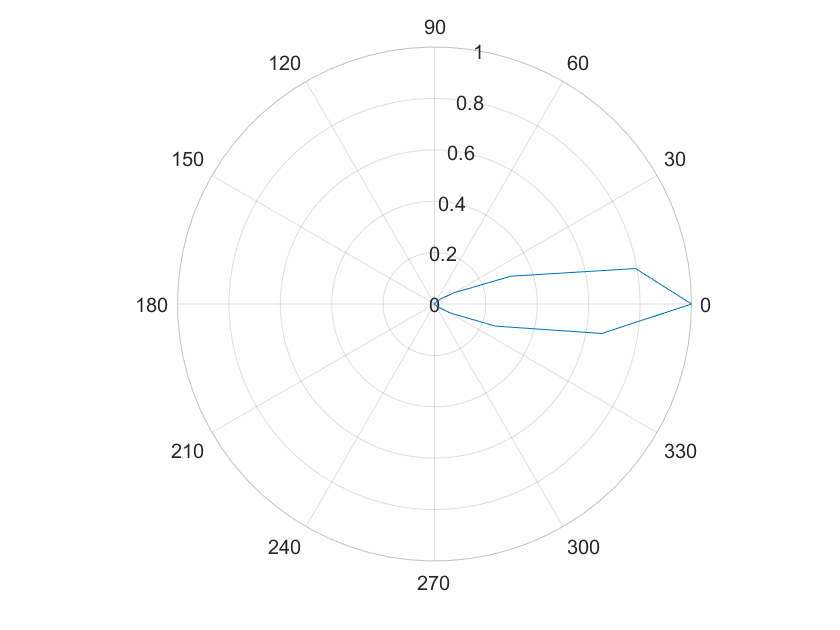
\includegraphics[width = \linewidth]{figure/水平方向图.png}
                    \caption{水平方向图}
                \end{minipage}
            }
            \subfigure[]{
                \begin{minipage}[t]{0.45\linewidth}

                \centering
                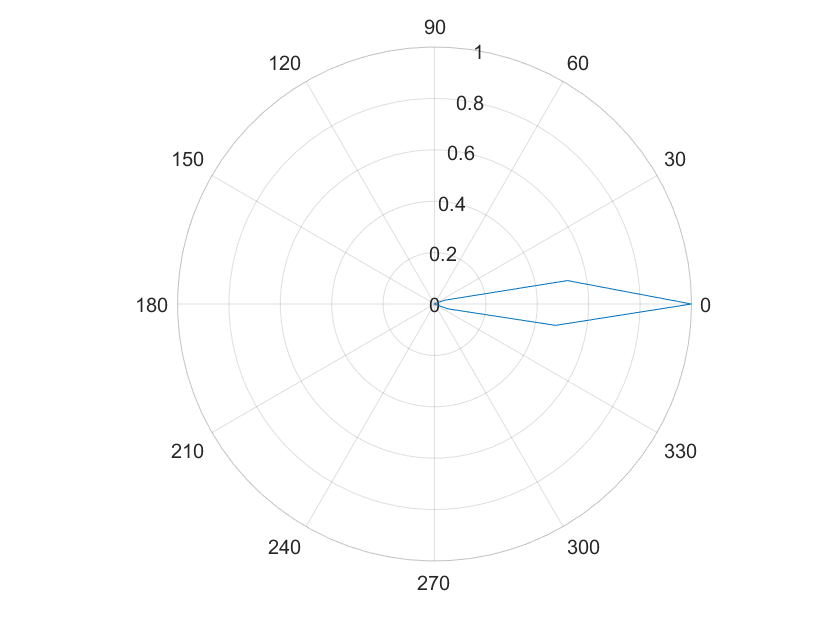
\includegraphics[width = \linewidth]{figure/垂直方向图.png}
                \caption{垂直方向图}
                                    
                \end{minipage}
            }
        \end{figure}

    \subsection{比较半功率波束宽度的计算值与实测值,并对你的实验结果加以评论。}
    测量值发射喇叭H面为25°,折合0.43rad,相比计算值0.46rad偏小

    测量值发射喇叭E面为35°,这个0.61rad,相比计算值0.77rad偏小

    \subsection{解释在$\pm$ 90°时辐射方向图测量值(提示:跟背景噪声比较)}
    在±90°的方向测得的结果并非为零,原因是背景噪声的干扰和发射处的电磁波在四周反射后被接收的结果

    \section{收获与体会}
    在天线辐射特性测量实验中,我验证了以前CST软件仿真出来的特性。在实践中认识到随着距离增加,衰减增强的关系,虽然这一规律因为其他组实验的干扰没有成功得出其与$\frac{1}{R^2}$之间的关系,但也从定性的角度了解到了这一规律。其次,后续的极化测量实验也让人更加直观地了解到了电磁场的极化;最后,天线的辐射方向图测量更是让人清晰地认识到了天线发射的信号具有方向性。

    实验极其容易受到外界干扰,人员应该注意分工,尽量不要随意走动,同时注意不要几组一起进行实验,我们测量与距离关系实验时,因为实验室内同时做实验的人员很多、各种电子设备之间相互干扰,带来了一定的误差。

\end{document}